\documentclass[11pt,a4paper]{article}
\usepackage[T1]{fontenc}
\usepackage[utf8]{inputenc}
\usepackage[margin=27mm,headheight=15pt]{geometry}
\usepackage{microtype}
\usepackage{amsmath,amsthm,mathtools}
\usepackage{newpxtext,newpxmath}
\usepackage{booktabs,array,longtable}
\usepackage{graphicx}
\usepackage[dvipsnames]{xcolor}
\usepackage{enumitem}
\usepackage{fancyhdr}
\usepackage{hyperref}
\usepackage{bookmark}
\hypersetup{colorlinks=true,linkcolor=MidnightBlue,citecolor=MidnightBlue,
 urlcolor=MidnightBlue,pdftitle={Theta Asymptotics for High-Power Ballot Sums},
 pdfauthor={Research article prepared with ChatGPT}}
\pagestyle{fancy}\fancyhf{}
\fancyhead[L]{\small Theta asymptotics for ballot sums}
\fancyhead[R]{\small OEIS A357825 and A357871}
\fancyfoot[C]{\thepage}
\renewcommand{\headrulewidth}{0.3pt}
\setlength{\parskip}{4pt}
\setlength{\parindent}{1.2em}
\setlist{itemsep=3pt,topsep=5pt}
\numberwithin{equation}{section}
\newtheorem{theorem}{Theorem}[section]
\newtheorem{proposition}[theorem]{Proposition}
\newtheorem{lemma}[theorem]{Lemma}
\newtheorem{corollary}[theorem]{Corollary}
\theoremstyle{definition}
\newtheorem{definition}[theorem]{Definition}
\newtheorem{remark}[theorem]{Remark}
\newcommand{\Z}{\mathbb Z}
\newcommand{\N}{\mathbb N}
\newcommand{\R}{\mathbb R}
\newcommand{\Acal}{\mathcal A}
\newcommand{\Bcal}{\mathcal B}
\newcommand{\bcont}{\mathfrak b}
\newcommand{\eps}{\varepsilon}
\newcommand{\dd}{\,\mathrm d}
\newcommand{\ee}{\mathrm e}
\newcommand{\OO}{\mathcal O}
\DeclareMathOperator{\dist}{dist}
\DeclareMathOperator{\Var}{Var}
\DeclareMathOperator{\TV}{TV}
\newcommand{\ind}{\mathbf 1}
\newcommand{\seq}[1]{\href{https://oeis.org/#1}{\texttt{#1}}}
\newcommand{\code}[1]{\texttt{#1}}
\setcounter{tocdepth}{2}
\begin{document}
\hypersetup{pageanchor=false}
\begin{titlepage}
\thispagestyle{empty}
\vspace*{7mm}
\noindent{\small\sffamily\color{MidnightBlue} RESEARCH ARTICLE \hfill 1 OCTOBER 2026}
\vspace{14mm}
\begin{flushleft}
{\Huge\bfseries Theta Asymptotics for\\[3pt] High-Power Ballot Sums\par}
\vspace{7mm}
{\Large OEIS A357825, A357871, and the\\growing-power array A357824\par}
\vspace{7mm}
{\large Exact oscillation envelopes, all-orders expansions,\\
exponential multiset corrections, and inverse asymptotics\par}
\end{flushleft}
\vspace{8mm}
\noindent\rule{\textwidth}{0.5pt}
\begin{abstract}
Let $B(n,h)$ count nonnegative unit-step paths of length $n$ ending at height
$h$, and let $a_n=\sum_h B(n,h)^n$. The OEIS records the leading root growth
of this sequence and the failure of a natural normalized ratio to converge.
We derive its missing multiplicative structure: the ratio is a Jacobi theta
function evaluated at a drifting parity-sensitive square-root phase, times
$\ee^{-5/6}$. A uniform all-orders expansion expresses every subsequent
coefficient as a Gaussian-weighted polynomial sum, equivalently a finite
linear combination of theta derivatives. We prove the exact lower and upper
limiting constants, identify the entire cluster interval and limiting phase
law, and obtain oscillatory adjacent-ratio and Tur\'an asymptotics. In
particular, the sequence is eventually strictly log-convex.

The multiset counterpart $b_n=\sum_h\binom{B(n,h)+n-1}{n}$ has the same
algebraic asymptotic expansion after multiplication by $n!$, but differs by
an explicitly determined first exponential sector of relative order
$n^3 2^{-n}$. An exact rising-factorial identity supplies every fixed
exponential sector. We also treat the array $\sum_hB(n,h)^k$: its transition
from a continuous Gaussian approximation to a finite-width lattice theta
sum occurs at $k\asymp n$. An exact two-endpoint estimate covers all larger
powers and yields a second, near-square logistic transition at
$k\asymp n^{3/2}$. Finally, we derive parity-sensitive inverse
expansions and explain their precise relation to integer thresholds.
The proofs are accompanied by independent exact integer checks, symbolic
coefficient generation, and high-precision numerical experiments.
\end{abstract}
\vfill
\noindent\fcolorbox{MidnightBlue}{MidnightBlue!3}{%
\begin{minipage}{0.94\textwidth}\small
\textbf{Status and scope.} This is a self-contained mathematical research
report, not a Lean formalization or an independently refereed paper.
The asymptotic formulas below are proved here; computational checks support
but do not replace those proofs. No claim of established publication
priority is made. The prime-power supercongruence recorded for A357825 is
\emph{not} resolved in this report.
\end{minipage}}\par
\vspace{5mm}
\noindent{\small Prepared with ChatGPT as a proposed contribution to the ProveIt research corpus.
[Write note, batch 73O1: filed in ProveIt's research-report collection;
provenance and status in Section~\ref{tbs:sec:collection}.]}
\end{titlepage}
\hypersetup{pageanchor=true}
\begingroup
\small
\setlength{\parskip}{0pt}
\tableofcontents
\endgroup
\newpage

\part{Theta asymptotics for high-power ballot sums}

\section{The question, the contribution, and its provenance}\label{tbs:sec:context}

\subsection{What the OEIS already records}
For a nonnegative integer $n$ and an admissible height
$h\in\{n,n-2,\ldots,n-2\lfloor n/2\rfloor\}$, put
\begin{equation}\label{tbs:eq:ballot}
 B(n,h)=\binom{n}{(n-h)/2}-\binom{n}{(n-h)/2-1},
\end{equation}
where a binomial coefficient with lower index $-1$ is zero. These are the
ballot numbers in \seq{A008315}. Reflection at the first visit to height
$-1$ gives the interpretation as nonnegative paths with steps $+1$ and
$-1$. Define
\begin{equation}\label{tbs:eq:definitions}
 S_{n,k}=\sum_h B(n,h)^k,\qquad
 a_n=S_{n,n},\qquad
 b_n=\sum_h\binom{B(n,h)+n-1}{n}.
\end{equation}
The array $S_{n,k}$ is \seq{A357824}, its diagonal $a_n$ is
\seq{A357825}, and $b_n$ is \seq{A357871}
\cite{oeisballot,oeisarray,oeisa,oeisb}. The powers count ordered tuples
sharing a common endpoint; the binomial coefficients count multisets
sharing a common endpoint. The first values are
\[
 (a_n)_{n=0}^6=(1,1,2,9,98,4150,562692),\qquad
 (b_n)_{n=0}^6=(1,1,2,5,21,183,3424).
\]

For $n\ge1$, set
\begin{align}
 K_n&=\frac{2^{n+3/2}}{\sqrt{\pi\ee}\,n},&
 \Acal_n&=K_n^n
 =\frac{2^{n^2+3n/2}}{\pi^{n/2}\ee^{n/2}n^n},\label{tbs:eq:normalizations-a}\\
 \Bcal_n&=\frac{\ee^{n/2}2^{n^2+3n/2}}
 {\pi^{n/2}n^{2n+1/2}}.\label{tbs:eq:normalizations-b}
\end{align}
Kotesovec's entries from November 2022 state $a_n^{1/n}\sim K_n$ and
that $a_n/\Acal_n$ has no limit. The multiset entry gives the analogous
root asymptotic and nonconvergence for $b_n/\Bcal_n$
\cite{oeisa,oeisb}. Those observations are the starting point, not claims
of this report's discovery. The natural next questions are: what replaces
the missing constant, how large are the oscillations, and is there a
uniform expansion beyond their leading shape?

\subsection{What is established here}
The main result is
\begin{equation}\label{tbs:eq:main-preview}
 \frac{a_n}{\Acal_n}
 =\ee^{-5/6}\!\left\{\Theta(\alpha_n)
 +\frac{F_1(\alpha_n)}{\sqrt{n+1}}
 +\frac{F_2(\alpha_n)}{n+1}+\cdots\right\},
\end{equation}
with a proved remainder after every fixed number of terms. Here
\[
 \alpha_n=\frac{\sqrt{n+1}-((n+1)\bmod2)}2,
 \qquad
 \Theta(\alpha)=\sum_{j\in\Z}\ee^{-4(j-\alpha)^2}.
\]
The coefficient functions are periodic and explicitly computable. The
oscillations are therefore organized by a simple phase, not erratic noise.
The main extensions are an exact limiting interval and distribution,
eventual log-convexity, the $k\asymp n$ transition for the entire array,
all fixed exponential sectors connecting the tuple and multiset counts,
and an inverse expansion retaining the same phase.

\begin{center}
\small
\begin{tabular}{@{}p{0.29\textwidth}p{0.64\textwidth}@{}}
\toprule
Question or assertion & Status in this report\\
\midrule
Root growth and absence of a limit & Already recorded by OEIS; proved and sharpened here.\\
Theta factor and every algebraic order & Explicit formulas with a uniform localization proof.\\
Multiset exponential corrections & Exact finite identity and every fixed-sector remainder.\\
Growing powers and inverse formulas & Proved in the parameter ranges stated below.\\
Global log-convexity at every index & Not claimed; only eventual strict log-convexity is proved.\\
Bala's prime-power supercongruence & Left open; no arithmetic conclusion is inferred from asymptotics.\\
Lean verification and publication priority & Neither is claimed.\\
\bottomrule
\end{tabular}
\end{center}

\subsection{Relation to the literature and ProveIt}
Catalan-triangle moments and fixed powers are part of an established
literature; Miana and Romero study such moments, closed expressions in
several cases, and divisibility questions \cite{miana}. The present
asymptotic regime instead lets the exponent grow with the row index.
Discrete Laplace methods are also established; a recent systematic
formulation is given by Helton, Hughes, and Schlosser \cite{discretelaplace}.
The point here is not to rename that method as new, but to retain the
lattice when its mesh does \emph{not} become small relative to the peak
width. Standard Stirling and theta identities are used with attribution
\cite{dlmfgamma,dlmfpolygamma,dlmftheta,dlmftransform}.

Repository inspection used ProveIt commit
\begin{center}\small\texttt{50f93367b2859b2727c34c68cf87684c101768cc}\end{center}
and its combinatorics map \cite{proveit}. No existing repository theorem is required for the
proofs below. This article is a proposed additional research case study;
it does not promote a repository computation into a formal theorem.
A repository code search for A357825 and targeted public searches for the
sequence identifiers and theta/high-power ballot asymptotics did not
identify a matching all-orders formula in the material reviewed. That is
a limited search result, not a proof of novelty. The source-status audit
and bibliography are dated 1 October 2026.

\subsection{Place in the ProveIt collection}\label{tbs:sec:collection}
\emph{[Write note, batch 73O1, 1 October 2026.]} This report is filed in
ProveIt's research-report collection, in the directory
\begin{center}\small
\nolinkurl{SetTheory/Cardinals/docs/reports/generating-functions-and-asymptotics/}\
\nolinkurl{oeis-sequence-asymptotics/a357825-theta-ballot-power-sums}.
\end{center}
Its README there is the guide to the files.

\emph{Provenance.} The report is built from one manuscript: manuscript~59
of batch~73 (cluster O1) of ProveIt's incoming-reports intake, the archive
\code{OEIS\_Theta\_Ballot\_Sums.zip}, which arrived in commit
\code{aa43cc555} and was placed by commit \code{9df4ba51a}. Its pin is the
commit \code{50f93367b} quoted above (the delivered source audit calls it
the ``inspected tree commit''; it is a commit). The text is printed as
delivered. The write changed only the label names, which now carry the
prefix \code{tbs:}, and added the notes marked \emph{[Write note]}. Nothing
was merged into it, and no other manuscript of the batch treats these
sequences.

\emph{Status.} The manuscript was prepared with ChatGPT. It is unrefereed,
and nothing in it is formalized in Lean or any other proof assistant. The
intake reran the shipped verifier on a copy (\code{code/verify.py --all},
exit code~0; the eight data files it writes equal the delivered ones,
up to line endings). It also
checked independently the first terms of $a_n$ and $b_n$, the two envelope
constants of Theorem~\ref{tbs:thm:envelope} to 20 digits, and the
expansion through $F_2$ against exact sums for $n=100,200,400,800$. It did
not re-derive every proof. The OEIS values and attributions quoted in the
article were not re-fetched by the intake; they are as the manuscript
inspected them on 1 October 2026.

\emph{Shipped layout.} The delivered \code{requirements.txt} is shipped as
\code{data/requirements.txt}, and \code{build.sh} as \code{code/build.sh};
the paths printed in Section~\ref{tbs:sec:computations} are the delivered
ones. The figure PDFs were regenerated by the intake with embedded
TrueType instead of Type~3 fonts, from the same data; see the README. The
delivered README, PDF and checksum list are not shipped.

\emph{Neighbouring material.} The same mechanism, a continuous saddle
whose lattice is kept when its mesh stays comparable to the peak width,
producing a theta multiplier, appears in two packages of ProveIt's
series-and-transseries collection, for different objects: the
$q$-multinomial package \nolinkurl{Theta_Resolved_Optimal_Truncation_q_Multinomial}
and the chapter ``Galois numbers and root-lattice theta sectors'' of
\nolinkurl{Combinatorial_Transseries_Inverses}. They are cited for comparison
only; no statement here depends on them, and none of theirs on this
report. The report
\nolinkurl{hankel-determinants/catalan-and-ballot/ballot-polynomial-hankel-determinants}
studies Hankel determinants of ballot moments, not growing powers. Bala's
supercongruence (question~Q9 of Section~\ref{tbs:sec:research}) remains
open.

\emph{[Write note, batch 98D, 5 October 2026.]} Since batch~98 the report
has two Parts. Part~I is manuscript~59 of batch~73, as described above.
Part~II (Section~\ref{tbs:lpt:sec:front}) prints a later manuscript, the
late batch-98 arrival \nolinkurl{ProveIt_OEIS_Lattice_Peak_Transfer_2026-10-05.zip}
(arrival \code{1ec443bc4}, placement \code{3b9458b31}), which answers
question~Q6 in a sufficient-hypothesis form: a general lattice-peak
transfer theorem, with an all-orders, a multidimensional and an inverse
version, of which Theorem~\ref{tbs:thm:critical} and the Mahonian
report's critical window are instances. Its labels carry the prefix
\code{tbs:lpt:}, and its provenance is in
Section~\ref{tbs:lpt:sec:provenance}. Nothing of Part~I was changed
except the Part heading and the notes dated 5 October 2026.

\section{The shifted ballot identity and the main theorem}\label{tbs:sec:main}

\subsection{Why the shift by one matters}
Put
\begin{equation}\label{tbs:eq:shift}
 m=n+1,\qquad r=h+1,\qquad \eps_n=m\bmod2\in\{0,1\}.
\end{equation}
Then $r$ ranges over the positive integers of parity $m$ with $r\le m$.
A binomial simplification gives the exact identity
\begin{equation}\label{tbs:eq:shifted-ballot}
 B(n,h)=\frac r m\binom{m}{(m-r)/2}.
\end{equation}
Define the continuous positive interpolation, only as an analytic tool,
by
\begin{equation}\label{tbs:eq:gamma-interpolation}
 \bcont_m(r)=\frac r m\,
 \frac{\Gamma(m+1)}
 {\Gamma((m-r)/2+1)\Gamma((m+r)/2+1)},\qquad 0<r\le m,
\end{equation}
and introduce
\begin{equation}\label{tbs:eq:V}
 V_m=\frac{2^m}{m}\sqrt{\frac2{\pi\ee}}
 =K_n\frac n m.
\end{equation}
The maximum of the leading continuous shape is at $r=\sqrt m$.
Writing
\begin{equation}\label{tbs:eq:phase-u}
 \alpha_n=\frac{\sqrt m-\eps_n}{2},\qquad
 u=r-\sqrt m=2(j-\alpha_n),
\end{equation}
turns the summation into a translated lattice of fixed spacing $2$.
The phase can be reduced modulo $1$ whenever a periodic function is
applied to it. Keeping $m=n+1$, rather than replacing it prematurely by
$n$, is necessary for the correct constant and correction terms.

\begin{definition}[Theta sums and Gaussian moments]
For $\tau>0$ and $p\ge0$, let
\begin{equation}\label{tbs:eq:theta}
 \Theta_\tau(\alpha)=\sum_{j\in\Z}\ee^{-4\tau(j-\alpha)^2},\qquad
 M_{p,\tau}(\alpha)=\sum_{j\in\Z}[2(j-\alpha)]^p
                         \ee^{-4\tau(j-\alpha)^2}.
\end{equation}
Write $\Theta=\Theta_1$ and $M_p=M_{p,1}$. These sums and all of their
phase derivatives converge absolutely and locally uniformly in $\tau>0$.
They are smooth, $1$-periodic functions of $\alpha$.
\end{definition}

\begin{theorem}[All-orders diagonal expansion]\label{tbs:thm:main}
There are explicitly computable polynomials $R_j\in\mathbb Q[u]$, with
$R_0=1$, $\deg R_j\le3j$, and
$R_j(-u)=(-1)^jR_j(u)$, such that for every fixed $J\ge0$,
\begin{equation}\label{tbs:eq:allorders}
 \frac{a_n}{\Acal_n}
 =\ee^{-5/6}\left\{
 \sum_{j=0}^J m^{-j/2}F_j(\alpha_n)
 +\OO_J\!\left(m^{-(J+1)/2}\right)\right\},
 \qquad m=n+1,
\end{equation}
where
\begin{equation}\label{tbs:eq:F}
 F_j(\alpha)=\sum_{\ell\in\Z}\ee^{-u_\ell^2}R_j(u_\ell),
 \qquad u_\ell=2(\ell-\alpha).
\end{equation}
The implied constant is independent of the phase. In particular
$F_0=\Theta$, and the same order holds as a relative error after division
by the leading term.
\end{theorem}

The first two correction polynomials are
\begin{align}
 R_1(u)&=\frac{u^3}{3}+\frac{2u}{3},\label{tbs:eq:R1}\\
 R_2(u)&=\frac{u^6}{18}-\frac{u^4}{36}
            +\frac{11u^2}{9}+\frac{13}{60}.\label{tbs:eq:R2}
\end{align}
Consequently
\begin{align}
 F_1&=\frac13M_3+\frac23M_1
       =\frac1{192}\Theta'''+\frac7{24}\Theta',\label{tbs:eq:F1-derivative}\\
 F_2&=\frac1{18}M_6-\frac1{36}M_4
                   +\frac{11}{9}M_2+\frac{13}{60}\Theta.\label{tbs:eq:F2}
\end{align}
All derivatives here are with respect to $\alpha$.
At integer and half-integer phases $F_1$ vanishes by symmetry. Away from
those phases an $m^{-1/2}$ term is generally present; restricting an ansatz
to integral powers of $1/n$ loses genuine information.

\begin{remark}[Meaning of ``all orders'']
Equation \eqref{tbs:eq:allorders} is a Poincar\'e asymptotic expansion: $J$ is
fixed while $n\to\infty$. No convergence of the infinite series, optimal
truncation theorem, or resurgent description is asserted. Because its
coefficients are periodic functions of a drifting phase, it is an
\emph{oscillatory} expansion, not an ordinary real logarithmic-exponential
transseries with constant coefficients. The additional exponential sectors
in Section~\ref{tbs:sec:multisets} give a separate, precise beyond-all-orders
statement.
\end{remark}

\section{Uniform localization and the proof of the expansion}\label{tbs:sec:proof}

\subsection{A Stirling expansion with a moving argument}
Define
\begin{equation}\label{tbs:eq:f}
 f(x)=\log x-\frac{x^2-1}{2},\qquad x>0.
\end{equation}
It has a unique maximum $0$ at $x=1$, with $f''(1)=-2$.
The logarithmic Stirling expansion for $\Gamma$ gives the following
uniform form.

\begin{lemma}[Uniform local logarithm]\label{tbs:lem:stirling}
For every compact interval $I\subset(0,\infty)$ and every integer $L\ge0$,
\begin{equation}\label{tbs:eq:log-stirling}
 \log\frac{\bcont_m(\sqrt m\,x)}{V_m}
 =f(x)+\sum_{\ell=1}^{L}A_\ell(x)m^{-\ell}
       +\OO_{I,L}(m^{-L-1}),\qquad x\in I,
\end{equation}
for all sufficiently large $m$. The estimate may be differentiated any
fixed number of times in $x$, after increasing the finite Stirling
truncation used to establish it. Here
\begin{align}\label{tbs:eq:Aformula}
 A_\ell(x)={}&-\frac{x^{2\ell+2}}{(2\ell+2)(2\ell+1)}
              +\frac{x^{2\ell}}{2\ell}\notag\\
 &+\sum_{j=1}^{\lfloor(\ell+1)/2\rfloor}
 \frac{B_{2j}}{2j(2j-1)}
 \left[
 \ind_{\ell=2j-1}
 -2^{2j}\binom{2\ell-2j}{2\ell-4j+2}
                      x^{2\ell-4j+2}
 \right],
\end{align}
where $B_{2j}$ denotes a Bernoulli number, with $B_2=1/6$.
\end{lemma}

\begin{proof}
Set $z=x/\sqrt m$, and insert the logarithmic Stirling formula into
\eqref{tbs:eq:gamma-interpolation}. The exponential part of the binomial
coefficient is controlled by
\[
 \frac{(1+z)\log(1+z)+(1-z)\log(1-z)}2
 =\sum_{q\ge1}\frac{z^{2q}}{2q(2q-1)}.
\]
Its $q=1$ term gives $-x^2/2$, and its higher terms give the first term
of \eqref{tbs:eq:Aformula}. The square-root prefactor contributes
$-\frac12\log(1-z^2)$, producing the second term.

For a Bernoulli term with $p=2j-1$, subtraction of the two denominator
corrections produces
\[
 \frac{B_{2j}}{2jp}\,m^{-p}
 \bigl[1-2^p\{(1-z)^{-p}+(1+z)^{-p}\}\bigr].
\]
The even Taylor coefficient of $z^{2k}$ in the braces is
$2\binom{p+2k-1}{2k}$. Setting $k=\ell-p$ yields the summation in
\eqref{tbs:eq:Aformula}. The leading prefactors, together with $r/m$, are
exactly $V_m\exp f(x)$.

For $x$ in a fixed compact interval, both denominator arguments are
$m/2+\OO(\sqrt m)$, hence are bounded below by a positive multiple of
$m$. Finite Stirling remainder bounds and finite Taylor remainders are
therefore uniform. The corresponding digamma and polygamma expansions
supply the same conclusion after any fixed number of differentiations;
see \cite{dlmfgamma,dlmfpolygamma}. This proves the finite asymptotic
statement, without requiring convergence of the displayed infinite
Taylor or Stirling series outside their use as coefficient generators.
\end{proof}

For example,
\begin{align}
 A_1(x)&=-\frac{x^4}{12}+\frac{x^2}{2}-\frac14,\notag\\
 A_2(x)&=-\frac{x^6}{30}+\frac{x^4}{4}-\frac{x^2}{3},\label{tbs:eq:Aexamples}\\
 A_3(x)&=-\frac{x^8}{56}+\frac{x^6}{6}-\frac{x^4}{3}+\frac1{24}.
 \notag
\end{align}
In particular $A_1(1)=1/6$ and $A_1'(1)=2/3$.

\subsection{A global Gaussian bound}
A local Stirling calculation alone does not justify exchanging an
asymptotic expansion with a sum whose range grows. The necessary tail
control follows from global concavity.

\begin{lemma}[Uniform Gaussian domination]\label{tbs:lem:gaussian}
There are constants $C,c>0$ such that, for all sufficiently large $n$ and
all $0<r\le m=n+1$,
\begin{equation}\label{tbs:eq:global-envelope}
 n\log\frac{\bcont_m(r)}{K_n}\le C-c(r-\sqrt m)^2.
\end{equation}
In particular the normalized summands of $a_n$ have a phase-uniform
summable Gaussian envelope.
\end{lemma}

\begin{proof}
Write $\ell_m(r)=\log\bcont_m(r)$. Direct differentiation gives
\begin{equation}\label{tbs:eq:concavity}
 \ell_m''(r)=-\frac1{r^2}
 -\frac14\left[
 \psi_1\!\left(\frac{m-r}2+1\right)
 +\psi_1\!\left(\frac{m+r}2+1\right)\right],
\end{equation}
where $\psi_1$ is the trigamma function. For $z>0$ its positive series
satisfies
\[
 \psi_1(z)=\sum_{q=0}^{\infty}(z+q)^{-2}
 \ge\int_0^\infty(z+t)^{-2}\dd t=\frac1z.
\]
The two arguments in \eqref{tbs:eq:concavity} sum to $m+2$, so their
reciprocals sum to at least $4/(m+2)$. Thus
$\ell_m''(r)\le-1/(m+2)$ everywhere on the stated interval.

Lemma~\ref{tbs:lem:stirling}, including its differentiated form, gives
\[
 \ell_m'(\sqrt m)=\frac{2}{3m^{3/2}}+\OO(m^{-5/2}),\qquad
 n\log\frac{\bcont_m(\sqrt m)}{K_n}=\OO(1).
\]
Taylor's theorem with the global upper bound on the second derivative
now gives, with $u=r-\sqrt m$,
\[
 n\log\frac{\bcont_m(r)}{K_n}
 \le C+\OO(m^{-1/2})u-\frac{n}{2(m+2)}u^2.
\]
Completing the square absorbs the linear term and proves
\eqref{tbs:eq:global-envelope}.
\end{proof}

For $|u|>m^{1/12}$, the total contribution is
\[\OO\!\left(\exp(-c' m^{1/6})\right),\]
uniformly in the lattice translate, by the Gaussian envelope. This is smaller than every fixed algebraic power of $m^{-1}$.
It also controls every fixed polynomial moment of the tails.

\subsection{The coefficient engine}
Let $t=m^{-1/2}$ and introduce a formal series in $t$ whose coefficients
are polynomials in $u$:
\begin{align}\label{tbs:eq:master}
 \mathscr L(t,u)={}&-1+(t^{-2}-1)
 \left[f(1+ut)+\sum_{\ell\ge1}A_\ell(1+ut)t^{2\ell}\right]
 +\sum_{\ell\ge1}\frac{t^{2\ell}}{\ell(\ell+1)}\notag\\
 ={}&-\frac56-u^2+\sum_{j\ge1}D_j(u)t^j.
\end{align}
Only finitely many terms are required to obtain any specified coefficient.
The last sum appears because
\begin{equation}\label{tbs:eq:normalization-shift}
 (m-1)\log(1-1/m)
 =-1+\sum_{\ell\ge1}\frac{m^{-\ell}}{\ell(\ell+1)}.
\end{equation}
Thus $\mathscr L$ generates precisely the expansion of
$n\log(\bcont_m(\sqrt m+u)/K_n)$.
The first exponent polynomials are
\begin{align}
 D_1(u)&=\frac{u^3}{3}+\frac{2u}{3},\notag\\
 D_2(u)&=-\frac{u^4}{4}+u^2+\frac{13}{60},\notag\\
 D_3(u)&=\frac{u^5}{5}-\frac{2u^3}{3}-\frac{8u}{15},\label{tbs:eq:Dexamples}\\
 D_4(u)&=-\frac{u^6}{6}+\frac{u^4}{6}
                         +\frac{2u^2}{3}+\frac{59}{420}.\notag
\end{align}
Exponentiation gives the exact polynomial recurrence
\begin{equation}\label{tbs:eq:Rrecurrence}
 R_0(u)=1,\qquad
 R_j(u)=\frac1j\sum_{i=1}^j iD_i(u)R_{j-i}(u)\quad(j\ge1).
\end{equation}
Indeed it is the coefficient recurrence for
$\exp(\sum_{i\ge1}D_i t^i)=\sum_{j\ge0}R_jt^j$.
Each $D_i$ has parity $i$ and degree at most $i+2$. Any product
contributing to weight $j$ therefore has degree at most $3j$ and parity
$j$, proving the structural assertions of Theorem~\ref{tbs:thm:main}.

The constant $-5/6$ is worth isolating. Raising the peak's Stirling
correction to the $n$th power contributes $+1/6$ to the logarithm.
Converting $V_m^n$ to $K_n^n$ contributes $-1$. Their sum is $-5/6$;
omitting either effect gives the wrong oscillation envelope.

\subsection{A summable remainder and completion of the proof}
Fix $J$. On $|u|\le m^{1/12}$, apply Lemma~\ref{tbs:lem:stirling} with a
finite truncation larger than the order needed for $t^{J+1}$, and apply
Taylor's theorem to the finitely many functions at $x=1+ut$. Since
$|ut|\le m^{-5/12}$, these Taylor expansions are uniform. The first
nonconstant perturbation of the Gaussian exponent is bounded by
$C t(1+|u|^3)$, which is $o(1)$ on this window. Finite Taylor's theorem
for the exponential consequently gives some integer $d_J$ and constants
$C_J,c_J>0$ such that
\begin{align}\label{tbs:eq:local-remainder}
 &\left|\left(\frac{\bcont_m(\sqrt m+u)}{K_n}\right)^n
 -\ee^{-5/6-u^2}\sum_{j=0}^Jm^{-j/2}R_j(u)\right|\notag\\
 &\hspace{25mm}\le C_Jm^{-(J+1)/2}(1+|u|)^{d_J}\ee^{-c_Ju^2}.
\end{align}
To see why increasing the Stirling truncation suffices, its remainder
before multiplication by $n$ is $\OO(m^{-L-1})$ uniformly for $x$ near
$1$; after multiplication it is $\OO(m^{-L})$. Choosing
$L\ge\lceil(J+1)/2\rceil$ and retaining the required Taylor terms makes
it no larger than the requested order, with any extra polynomial factors
absorbed into $(1+|u|)^{d_J}$. The finitely many exponentiation remainders
have the same form.

For every $p\ge0$ and $c>0$,
\[
 \sup_{\alpha\in[0,1]}
 \sum_{j\in\Z}(1+|2(j-\alpha)|)^p\ee^{-c[2(j-\alpha)]^2}<\infty.
\]
Summing \eqref{tbs:eq:local-remainder} over the translated lattice therefore
preserves its algebraic order. Lemma~\ref{tbs:lem:gaussian} controls the
omitted actual summands outside the window. The polynomial-Gaussian
approximants have tails of the same negligible kind. Extending the
finite admissible lattice to all of $\Z$ adds only such tails, since both
endpoints are a growing distance from $\sqrt m$. This proves
\eqref{tbs:eq:allorders}. Finally, the nearest lattice point has $|u|\le1$,
so $\Theta(\alpha)\ge\ee^{-1}$ uniformly; absolute and relative versions
of the theorem are equivalent. \hfill$\square$

\section{Theta geometry, exact envelopes, and phase distribution}\label{tbs:sec:theta}

\subsection{Theta identities and extrema}
Poisson summation of a Gaussian gives
\begin{equation}\label{tbs:eq:poisson}
 \Theta_\tau(\alpha)=\frac{\sqrt\pi}{2\sqrt\tau}
 \sum_{q\in\Z}\exp\!\left(-\frac{\pi^2q^2}{4\tau}\right)
                         \ee^{2\pi i q\alpha}.
\end{equation}
This also follows from the standard theta transformation
\cite{dlmftransform}. Termwise differentiation of \eqref{tbs:eq:theta} gives
\begin{equation}\label{tbs:eq:momentrec}
 M_{p,\tau}'=-2pM_{p-1,\tau}+4\tau M_{p+1,\tau}.
\end{equation}
For $\tau=1$, iteration expresses every $F_j$ as a finite rational
linear combination of derivatives of $\Theta$. This is an alternative
all-orders representation to the rapidly convergent moment sums.

\begin{lemma}[Strict extrema]\label{tbs:lem:theta-extrema}
For each $\tau>0$, $\Theta_\tau$ is strictly decreasing on $(0,1/2)$.
Its global maximum is at integer phases and its global minimum is at
half-integer phases.
\end{lemma}
\begin{proof}
Let $q=\exp(-\pi^2/(4\tau))\in(0,1)$. Apart from the positive constant
in \eqref{tbs:eq:poisson}, the Jacobi product is
\[
 \prod_{j\ge1}(1-q^{2j})
 \bigl(1+2q^{2j-1}\cos(2\pi\alpha)+q^{4j-2}\bigr).
\]
Every phase-dependent factor is positive. Its logarithmic derivative is
strictly negative when $0<\alpha<1/2$. The derivative series converges
locally uniformly there, so the logarithmic derivative of the product
is negative. Periodicity and reflection symmetry finish the proof.
The product identity is standard \cite{dlmftheta}.
\end{proof}

\begin{theorem}[Exact limiting interval]\label{tbs:thm:envelope}
The cluster set of $a_n/\Acal_n$ is precisely $[C_-,C_+]$, where
\begin{align}
 C_-&=\ee^{-5/6}\sum_{j\in\Z}\ee^{-(2j-1)^2}
       =0.31986675953099572612\ldots,\label{tbs:eq:Cminus}\\
 C_+&=\ee^{-5/6}\sum_{j\in\Z}\ee^{-4j^2}
       =0.45051819401966197435\ldots.\label{tbs:eq:Cplus}
\end{align}
In particular these are respectively the liminf and limsup, and no
constant $C$ satisfies $a_n\sim C\Acal_n$.
\end{theorem}
\begin{proof}
Theorem~\ref{tbs:thm:main} reduces the claim to the range of $\Theta$ along
the phases. Lemma~\ref{tbs:lem:theta-extrema} supplies universal limiting
bounds. For $n=s^2-1$, the phase is an integer exactly, so this subsequence
converges to $C_+$. For $n=s^2$, the phase tends modulo one to $1/2$, so
that subsequence converges to $C_-$. Proposition~\ref{tbs:prop:equidist}
below proves that every phase occurs as a subsequential limit. Continuity
of $\Theta$ then fills the entire interval and excludes other cluster
values.
\end{proof}

\begin{figure}[tb]
\centering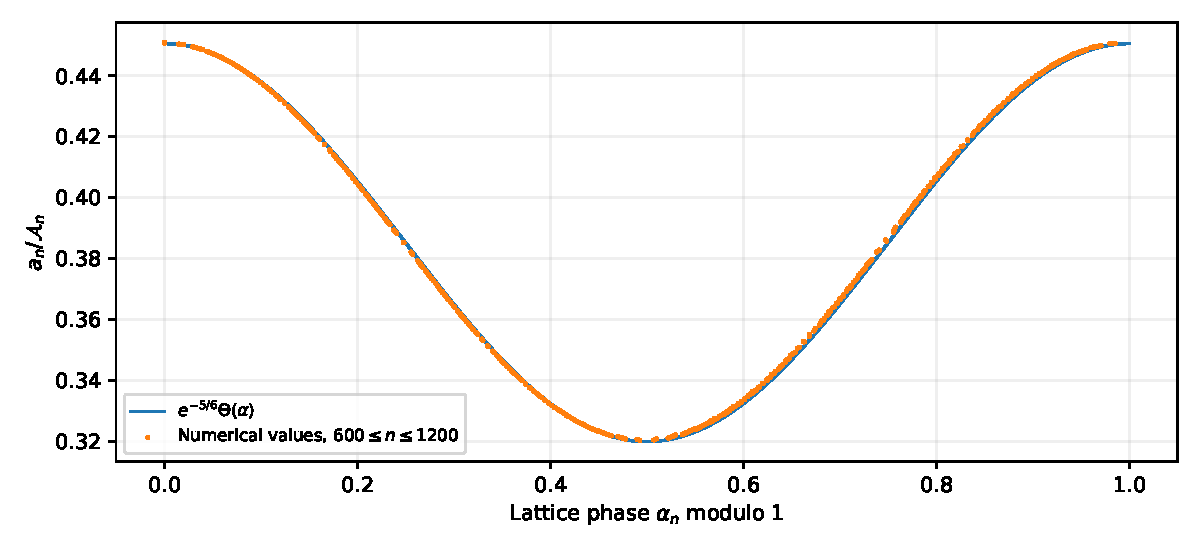
\includegraphics[width=0.97\textwidth]{figures/phase_collapse.pdf}
\caption{The apparent oscillation collapses onto a single theta curve
when plotted against the phase. Dots are high-precision localized
log-Gamma evaluations for $600\le n\le1200$, not interval-certified
values. The discrepancy is explained by the $m^{-1/2}$ and higher terms.}
\label{tbs:fig:phase}
\end{figure}

\subsection{An elementary equidistribution proof}
\begin{proposition}[Effective phase distribution]\label{tbs:prop:equidist}
For every interval $I\subset[0,1)$,
\begin{equation}\label{tbs:eq:equidist}
 \#\{1\le n\le N:\{\alpha_n\}\in I\}
 =N|I|+\OO(\sqrt N).
\end{equation}
The implied constant can be chosen independently of $I$. The same
assertion holds on either parity class, with its own number of terms
in place of $N$.
\end{proposition}
\begin{proof}
Fix $\eps\in\{0,1\}$ and restrict $m=n+1$ to that parity. For
$I=[a,b)$, the condition is equivalent to membership in the union of
intervals
\[
 (2j+\eps+2a)^2\le m<(2j+\eps+2b)^2,
\]
apart from finitely many harmless initial endpoints. The number of
integers of a specified parity in an interval of length $L$ is
$L/2+\OO(1)$. The displayed interval has length
\[
 8j(b-a)+4\eps(b-a)+4(b^2-a^2).
\]
There are $\OO(\sqrt N)$ complete intervals up to $N+1$.
Summing their main terms gives $(b-a)$ times the number of admissible
$m$ up to $N+1$, with error $\OO(\sqrt N)$: the terms linear in $j$
produce the quadratic main term, and all endpoint and linear-size
corrections are of order $\sqrt N$. A final partial interval also has
length $\OO(\sqrt N)$ and obeys the same bound. All constants are
uniform for $0\le a\le b\le1$. Summing the two parity classes proves
\eqref{tbs:eq:equidist}.
\end{proof}

\begin{corollary}[Limiting law and mean]\label{tbs:cor:law}
If an index is chosen uniformly from $1,\ldots,N$, then
$a_n/\Acal_n$ converges in distribution to $\ee^{-5/6}\Theta(U)$,
where $U$ is uniform on $[0,1]$. Moreover
\begin{equation}\label{tbs:eq:mean}
 \frac1N\sum_{n=1}^N\frac{a_n}{\Acal_n}
 =\ee^{-5/6}\frac{\sqrt\pi}{2}+\OO(N^{-1/2})
 =0.38515263413250459606\ldots+\OO(N^{-1/2}).
\end{equation}
\end{corollary}
\begin{proof}
Continuity and equidistribution prove convergence in distribution.
Integrating the discrepancy bound against the smooth function
$\Theta$ gives an $\OO(N^{-1/2})$ error in its average. The average of
the uniform $\OO(n^{-1/2})$ remainder in Theorem~\ref{tbs:thm:main} has the
same order. Finally
\[
 \int_0^1\Theta(\alpha)\dd\alpha
 =\frac12\int_{-\infty}^{\infty}\ee^{-u^2}\dd u
 =\frac{\sqrt\pi}{2}.
\]
\end{proof}

The root asymptotic in the OEIS follows immediately: $a_n/\Acal_n$ is
bounded above and bounded away from zero, so
$a_n^{1/n}/K_n=(a_n/\Acal_n)^{1/n}\to1$.
The multiplicative oscillation survives in the ratio but disappears
under the $n$th root.

\section{Adjacent quotients, log-convexity, and recurrence obstructions}\label{tbs:sec:ratios}

Put
\begin{equation}\label{tbs:eq:g}
 \lambda=\log2,\qquad c=\frac32\log2-\frac{1+\log\pi}{2},\qquad
 g(x)=\lambda x^2-x\log x+cx.
\end{equation}
Then $g(n)=\log\Acal_n$. Consecutive phases satisfy
\begin{equation}\label{tbs:eq:adjacent-phase}
 \alpha_{n\pm1}=\alpha_n+\frac12+\OO(n^{-1/2})\pmod1.
\end{equation}
Thus averaging away the phase before forming an adjacent quotient would
lose an order-one factor.

\begin{theorem}[Adjacent and Tur\'an quotients]\label{tbs:thm:ratios}
As $n\to\infty$,
\begin{align}
 \frac{a_{n+1}}{a_n}
 &=\frac{2^{2n+5/2}}{\sqrt\pi\,\ee^{3/2}n}
   \frac{\Theta(\alpha_n+1/2)}{\Theta(\alpha_n)}
   \bigl(1+\OO(n^{-1/2})\bigr),\label{tbs:eq:adjacent-ratio}\\
 \frac{a_{n-1}a_{n+1}}{a_n^2}
 &=4\left(\frac{\Theta(\alpha_n+1/2)}{\Theta(\alpha_n)}\right)^2
   +\OO(n^{-1/2}).\label{tbs:eq:turan}
\end{align}
The second quotient has lower and upper limits
\begin{align}
 T_-&=4\left(\frac{\Theta(1/2)}{\Theta(0)}\right)^2
       =2.01638539749423251125\ldots,\label{tbs:eq:turan-lower}\\
 T_+&=4\left(\frac{\Theta(0)}{\Theta(1/2)}\right)^2
       =7.93499100910135656311\ldots.\label{tbs:eq:turan-upper}
\end{align}
In particular $a_n$ is strictly log-convex for all sufficiently large $n$.
\end{theorem}
\begin{proof}
Taylor expansion of $g$ gives
\[
 \ee^{g(n+1)-g(n)}
 =\frac{2^{2n+5/2}}{\sqrt\pi\,\ee^{3/2}n}(1+\OO(n^{-1})),
 \qquad
 \ee^{g(n-1)+g(n+1)-2g(n)}=4(1+\OO(n^{-1})).
\]
Use Theorem~\ref{tbs:thm:main}, \eqref{tbs:eq:adjacent-phase}, smoothness, and
positivity of $\Theta$. The ratio of two theta values is bounded by
$\Theta(1/2)/\Theta(0)$ and its reciprocal. Both bounds are attained at
phases $0$ and $1/2$, which occur as subsequential limits.

The strict inequality $T_->1$ need not rest on floating-point decimals.
For instance $\Theta(1/2)\ge2/\ee>2/3$, while
\[
 \Theta(0)=1+2\sum_{j\ge1}\ee^{-4j^2}
 \le1+\frac{2\ee^{-4}}{1-\ee^{-12}}<\frac{11}{10}.
\]
The last elementary bound follows already from $\ee>8/3$.
Consequently $T_->4(20/33)^2>1$, a positive gap from the
log-convexity threshold. Equation \eqref{tbs:eq:turan} proves the final
assertion.
\end{proof}

A rapidly growing sequence need not automatically be log-convex:
oscillatory multipliers can interfere with a second difference. Here the
theta quotient is explicitly controlled, so the conclusion has a genuine
proof rather than following from growth alone. The theorem does not
specify the least index from which log-convexity holds.

\begin{proposition}[No polynomial-coefficient linear recurrence]\label{tbs:prop:nonprecursive}
Neither $(a_n)$ nor $(b_n)$ is P-recursive over $\mathbb C$. Equivalently,
neither ordinary generating series is D-finite as a formal power series.
Both ordinary generating series have radius of convergence zero.
\end{proposition}
\begin{proof}
A sequence $u_n$ satisfying a nonzero polynomial-coefficient recurrence
$\sum_{j=0}^r p_j(n)u_{n+j}=0$ can, for all large $n$, be solved for the
term with largest nonzero index. Ratios of its polynomial coefficients
are bounded in magnitude by $Cn^d$ for some integer $d\ge0$.
If $M_N=\max(1,|u_0|,\ldots,|u_N|)$, it follows that
$M_{N+1}\le C' N^dM_N$ after adjusting constants and ignoring a finite
initial segment. Hence
\[
 |u_n|\le C_0C_1^n(n!)^d,\qquad \log^+|u_n|=\OO(n\log n).
\]
A recurrence of order zero would force eventual vanishing and is also
impossible here. Theorem~\ref{tbs:thm:main} gives
$\log a_n=\lambda n^2+\OO(n\log n)$. Theorem~\ref{tbs:thm:sectors}
below gives the same quadratic leading logarithm for $b_n$.
Both contradict the recurrence bound. The equivalence with formal
D-finiteness follows by coefficient extraction from a linear differential
equation and the converse conversion of a recurrence to such an equation.
Finally $a_n^{1/n}$ and $b_n^{1/n}$ tend to infinity, so the radius
assertion follows from the root test.
\end{proof}

\section{The growing-power array and two localization transitions}\label{tbs:sec:array}

The scale of the exponent determines whether the lattice can be replaced
by an integral. This section treats $S_{n,k}$ for real $k>0$ analytically;
integer $k$ gives the OEIS array. The parameter $m=n+1$ is always retained.

\subsection{Fixed powers and the broad Gaussian regime}
\begin{proposition}[Fixed and subcritical powers]\label{tbs:prop:subcritical}
For each fixed $k>0$,
\begin{equation}\label{tbs:eq:fixed-k}
 S_{n,k}\sim V_m^k\frac{\sqrt m}{4}\,
 \ee^{k/2}\left(\frac2k\right)^{(k+1)/2}
 \Gamma\!\left(\frac{k+1}{2}\right).
\end{equation}
If $k=k(n)\to\infty$ and $k=o(m)$, then
\begin{equation}\label{tbs:eq:subcritical}
 S_{n,k}\sim V_m^k\frac{\sqrt{\pi m/k}}2.
\end{equation}
\end{proposition}
\begin{proof}
For fixed $k$, use $x=r/\sqrt m$. Its lattice mesh is $2/\sqrt m$.
Lemma~\ref{tbs:lem:stirling} gives pointwise convergence of
$(\bcont_m(\sqrt m x)/V_m)^k$ to
$\ee^{kf(x)}=\ee^{k/2}x^k\ee^{-kx^2/2}$. The concavity proof gives a
uniform integrable Gaussian bound in $x-1$; compact-interval convergence
and this tail bound justify the Riemann sum. Thus
\[
 S_{n,k}/V_m^k\sim\frac{\sqrt m}{2}\int_0^\infty
          \ee^{k/2}x^k\ee^{-kx^2/2}\dd x,
\]
whose integral is \eqref{tbs:eq:fixed-k}.

For growing $k=o(m)$, use the finer local variable
$v=(r-\sqrt m)\sqrt{k/m}$. The mesh $2\sqrt{k/m}$ tends to zero,
while
\[
 kf(1+v/\sqrt k)\longrightarrow-v^2,
 \qquad kA_1(1+v/\sqrt k)/m\longrightarrow0
\]
uniformly for bounded $v$. The same concavity argument gives a uniform
Gaussian tail in $v$. The Riemann-sum limit is therefore
$\frac12\sqrt{m/k}\int_{\R}\ee^{-v^2}\dd v$, proving
\eqref{tbs:eq:subcritical}.
\end{proof}

For orientation, the first two integral powers also have exact familiar
identities:
\[
 S_{n,1}=\binom{n}{\lfloor n/2\rfloor},\qquad
 S_{n,2}=\frac1{n+1}\binom{2n}{n}.
\]
The first telescopes in \eqref{tbs:eq:ballot}. For the second, join a pair of
nonnegative $n$-step paths with common height by following the first and
then the reverse of the second. This is a bijection with Dyck paths of
length $2n$. These columns are already identified by the OEIS
\cite{oeisarray}; they are consistency checks, not new enumeration claims.

\subsection{The critical theta regime}
\begin{theorem}[Critical growing powers]\label{tbs:thm:critical}
Let $\tau=k/m$ stay in a compact subinterval of $(0,\infty)$. Uniformly
in $\tau$ and in the phase,
\begin{equation}\label{tbs:eq:critical}
 S_{n,k}=V_m^k\ee^{\tau/6}
 \left[\Theta_\tau(\alpha_n)+\OO(m^{-1/2})\right].
\end{equation}
There is an expansion to every fixed order in $m^{-1/2}$, with
coefficients that are polynomial-Gaussian sums and smooth in $\tau$.
Its first correction inside the brackets is
\begin{equation}\label{tbs:eq:critical-first}
 \frac{\tau}{\sqrt m}\sum_{j\in\Z}
 \left(\frac{u_j^3}{3}+\frac{2u_j}{3}\right)\ee^{-\tau u_j^2},
 \qquad u_j=2(j-\alpha_n).
\end{equation}
\end{theorem}
\begin{proof}
Replace the factor $n=m-1$ in the local logarithmic analysis by
$k=\tau m$. Lemma~\ref{tbs:lem:stirling} gives
\[
 k\log\frac{\bcont_m(\sqrt m+u)}{V_m}
 =\tau\left(\frac16-u^2\right)
 +\frac{\tau}{\sqrt m}\left(\frac{u^3}{3}+\frac{2u}{3}\right)
 +\OO\!\left(m^{-1}(1+|u|)^4\right)
\]
on bounded windows, uniformly for $\tau$ in the given compact interval.
All higher coefficients follow by the same finite Taylor procedure.
The global concavity bound, now multiplied by $k$, gives a summable
Gaussian with constants uniform on that interval. The argument of
\eqref{tbs:eq:local-remainder} therefore applies without change.
\end{proof}

The width in $r$ is of order $\sqrt{m/k}$. It is large in
\eqref{tbs:eq:subcritical}, but of order one in \eqref{tbs:eq:critical}.
This explains the first localization transition, $k\asymp m$.
\emph{[Write note, batch 98D, 5 October 2026: the leading term of
Theorem~\ref{tbs:thm:critical} is an instance of Part~II's general
transfer theorem (Theorem~\ref{tbs:lpt:thm:transfer} with
Proposition~\ref{tbs:lpt:prop:ballot}), with $q=8\tau$.]}

For a probabilistic formulation, choose an endpoint with probability
$\mathbb P_{n,k}(h)=B(n,h)^k/S_{n,k}$. After writing $u=h+1-\sqrt m$,
the critical law is approximated in total variation, with error
$\OO(m^{-1/2})$, by the phase-shifted discrete Gaussian
\begin{equation}\label{tbs:eq:discrete-law}
 \mathbb P\{u=2(j-\alpha_n)\}
 =\frac{\ee^{-4\tau(j-\alpha_n)^2}}{\Theta_\tau(\alpha_n)}.
\end{equation}
Here the comparison extends the admissible finite lattice to all integers;
the added tail is negligible. The weighted remainder bound in the proof
also yields
\begin{equation}\label{tbs:eq:mean-endpoint}
 \mathbb E_{n,k}[h+1-\sqrt m]
 =\frac{\Theta_\tau'(\alpha_n)}{4\tau\Theta_\tau(\alpha_n)}
  +\OO(m^{-1/2}).
\end{equation}
The limit is not a single continuous Gaussian: subsequences with different
phases have different discrete endpoint laws.

\subsection{Exact modes and a uniform two-endpoint theorem}
An exact ratio gives more than a truncated Stirling approximation in the
supercritical regime. From \eqref{tbs:eq:shifted-ballot},
\begin{equation}\label{tbs:eq:exact-ratio}
 \rho_m(r):=\frac{(r+2)(m-r)}{r(m+r+2)},\qquad 0<r<m.
\end{equation}
It equals $\bcont_m(r+2)/\bcont_m(r)$ when both arguments lie in
$(0,m]$, and equals $1$ exactly when $m=r(r+2)$.

\begin{theorem}[Exact modes and all supercritical powers]\label{tbs:thm:two-sites}
For $m\ge3$, set $y=\sqrt{m+1}$, and let $r_-$ be the largest positive
integer of parity $m$ satisfying $r_-\le y$. Put $r_+=r_-+2$ and
$W_\pm=\bcont_m(r_\pm)$.

The maximum ballot entry occurs at the admissible $r$ nearest to $y$.
There are exactly two tied maxima if and only if $m+1=s^2$ for an integer
$s\ge2$; then their locations are $r=s-1,s+1$.
For every real $k>0$,
\begin{equation}\label{tbs:eq:two-site-bound}
 0\le\frac{S_{n,k}}{W_-^k+W_+^k}-1
 \le\sum_{\ell\ge1}\exp\!\left(-\frac{2k\ell^2}{m+1}\right).
\end{equation}
Consequently, whenever $k/m\to\infty$, with \emph{no upper bound} on $k$,
\begin{equation}\label{tbs:eq:supercritical-exact}
 S_{n,k}=(W_-^k+W_+^k)
 \left[1+\OO\!\left(\ee^{-2k/(m+1)}\right)\right],
\end{equation}
uniformly in the phase.
\end{theorem}
\begin{proof}
The sign of $\rho_m(r)-1$ is the sign of $m-r(r+2)$, so adjacent
entries increase up to the midpoint criterion $r+1=y$ and decrease
after it. This proves the nearest-point and exact-tie statements.
The candidate pair lies within $0<r\le m$ for $m\ge3$.

For the uniform remainder, differentiate the logarithm of the exact
ratio:
\begin{align*}
 \frac{\dd}{\dd r}\log\rho_m(r)
 &=-\frac{2}{r(r+2)}-\frac1{m-r}-\frac1{m+r+2}\\
 &\le-\frac{2}{m+1},\qquad 0<r<m.
\end{align*}
The last inequality follows because
$(m-r)(m+r+2)=(m+1)^2-(r+1)^2\le(m+1)^2$.
Also $\log\rho_m(y-1)=0$.

For the $i$th ratio to the left of $r_-$, the distance from its argument
$r_--2i$ to $y-1$ is at least $2i-1$. Integrating the derivative bound
and summing the ratios therefore gives
\[
 \frac{\bcont_m(r_--2\ell)}{W_-}
 \le\exp\!\left(-\frac{2\ell^2}{m+1}\right)
\]
whenever that lattice point is admissible. The ratios to the right of
$r_+$ obey the same estimate relative to $W_+$. Raising to $k$ and
summing both tails proves \eqref{tbs:eq:two-site-bound}. Finally, with
$t=k/(m+1)$,
\[
 \sum_{\ell\ge1}\ee^{-2t\ell^2}
 \le\frac{\ee^{-2t}}{1-\ee^{-6t}},
\]
which proves the claimed supercritical order as $t\to\infty$.
\end{proof}

This theorem keeps the two dominant ballot entries \emph{exact}. It is
therefore valid even when errors from raising a Stirling approximation
to an extremely large power would be unacceptable. It also identifies a
small but consequential distinction: the leading continuous saddle is
$\sqrt m$, whereas the exact discrete mode is selected by
$\sqrt{m+1}$. A shift negligible at $k\asymp m$ need not be negligible
at a much larger exponent.

The two main terms can equivalently be written
\begin{equation}\label{tbs:eq:cosh-exact}
 W_-^k+W_+^k
 =2(W_-W_+)^{k/2}\cosh\!\left(\frac{k}{2}
                         \log\frac{W_+}{W_-}\right).
\end{equation}
Thus the precise crossover is governed by $k\log(W_+/W_-)$, not by an
uncontrolled choice of one approximate maximum.

\subsection{A second transition near square-index ties}
\begin{corollary}[Near-square logistic limit]\label{tbs:cor:logistic}
Fix an integer $d$ and $\kappa>0$. Along
\begin{equation}\label{tbs:eq:square-window}
 n=s^2-2+2d,\qquad k/s^3\longrightarrow\kappa,
 \qquad s\to\infty,
\end{equation}
the endpoint law concentrates on $h=s-2$ and $h=s$, and
\begin{equation}\label{tbs:eq:logistic}
 \mathbb P_{n,k}\{h=s\}\longrightarrow
 \frac{1}{1+\ee^{-4\kappa d}},\qquad
 \mathbb P_{n,k}\{h=s-2\}\longrightarrow
 \frac{1}{1+\ee^{4\kappa d}}.
\end{equation}
For $k=\kappa s^3+\OO(1)$ the errors are $\OO(s^{-2})$.
\end{corollary}
\begin{proof}
For fixed $d$ and large $s$, the bracketing admissible points are
$r_-=s-1$ and $r_+=s+1$. The factor $2d$ in
\eqref{tbs:eq:square-window} preserves their parity; replacing it by an
arbitrary odd shift would change the endpoint lattice. Substitution into
\eqref{tbs:eq:exact-ratio} gives the exact identity
\begin{equation}\label{tbs:eq:square-ratio}
 \frac{W_+}{W_-}
 =1+\frac{4d}{(s-1)(s^2+s+2d)},
 \qquad
 \log\frac{W_+}{W_-}=\frac{4d}{s^3}+\OO_d(s^{-5}).
\end{equation}
Since $k/m\sim\kappa s\to\infty$,
Theorem~\ref{tbs:thm:two-sites} makes the other endpoints exponentially
negligible. The upper endpoint probability is therefore
$\rho^k/(1+\rho^k)$ plus an exponentially small error. Equation
\eqref{tbs:eq:square-ratio} yields \eqref{tbs:eq:logistic} and its error bound.
\end{proof}

The first transition, at $k\asymp n$, changes a broad Gaussian sum into
a finite-width lattice sum. The second, at $k\asymp n^{3/2}$ near
square-index ties, resolves two neighboring entries whose logarithms
differ by only order $n^{-3/2}$. At $d=0$ the exact tie persists and the
two limiting probabilities are $1/2$. This second transition is not an
assumption about the phase: it follows from the exact ballot ratio.

\section{Multisets and exponentially small sectors}\label{tbs:sec:multisets}

\subsection{An exact bridge between the two sequences}
Let $E_q(n)=e_q(0,1,\ldots,n-1)$ be an elementary symmetric polynomial,
so that
\begin{equation}\label{tbs:eq:rising}
 \prod_{j=0}^{n-1}(X+j)=\sum_{q=0}^{n}E_q(n)X^{n-q}.
\end{equation}
In particular $E_0=1$, $E_1=\binom n2$, and $E_n=0$ for $n\ge1$.
Multiplying each multiset binomial by $n!$ and summing yields the exact
identity
\begin{equation}\label{tbs:eq:sector-identity}
 \boxed{\displaystyle n!b_n=
       \sum_{q=0}^{n}E_q(n)S_{n,n-q}.}
\end{equation}
This identity separates the dominant tuple count from its successive
corrections without approximating individual small ballot entries.

\begin{theorem}[Every fixed exponential sector]\label{tbs:thm:sectors}
For each fixed $Q\ge0$, as $n\to\infty$,
\begin{equation}\label{tbs:eq:sector-remainder}
 \frac{n!b_n}{a_n}
 =\sum_{q=0}^{Q}E_q(n)\frac{S_{n,n-q}}{a_n}
 +\OO_Q\!\left(n^{2Q+2}V_m^{-Q-1}\right).
\end{equation}
For each fixed $q$, the quotient $S_{n,n-q}/a_n$ has a phase-uniform
expansion to every algebraic order, with leading term $V_m^{-q}$.
Thus \eqref{tbs:eq:sector-remainder} is an expansion in successive
exponentially small scales, each with its own algebraic expansion.
\end{theorem}
\begin{proof}
Nonnegativity and the multinomial expansion give
\[
 0\le E_q(n)\le\frac{E_1(n)^q}{q!}.
\]
For $0\le q\le n/2$, Theorems~\ref{tbs:thm:main} and \ref{tbs:thm:critical},
uniformly for the exponent ratio in a fixed interval around $[1/2,1]$,
imply
\[
 \frac{S_{n,n-q}}{a_n}\le C V_m^{-q}.
\]
For the remaining indices, let $M$ be the largest ballot entry. The
nearest-point estimate and the local expansion give
$M/V_m=\exp(\OO(1/m))$. Since there are at most $n+1$ summands and
$a_n\ge M^n$,
\[
 \frac{S_{n,n-q}}{a_n}\le(n+1)M^{-q}\le CnV_m^{-q}.
\]
Put $x=E_1/V_m$, which tends to zero exponentially. Summing the first
bound over $q\ge Q+1$ through $n/2$ gives $\OO_Q(x^{Q+1})$.
The remaining tail is at most
$Cn\sum_{q>n/2}x^q/q!$, smaller than every fixed power of $x$ for large
$n$. The exact identity \eqref{tbs:eq:sector-identity} proves the remainder.

For fixed $q$, apply the all-orders form of Theorem~\ref{tbs:thm:critical}
with $\tau=(n-q)/m=1-(q+1)/m$ and Taylor-expand its smooth coefficient
functions in $\tau$. Divide by the positive all-orders denominator from
Theorem~\ref{tbs:thm:main}. Formal series division is justified at each
finite order because the leading theta factor is bounded below.
The leading factors cancel except for $V_m^{-q}$.
\end{proof}

\subsection{The first sector and its phase correction}
\begin{theorem}[Explicit leading multiset correction]\label{tbs:thm:first-sector}
Let
\begin{equation}\label{tbs:eq:Lambda}
 \Lambda(\alpha)=\frac{M_2(\alpha)}{\Theta(\alpha)}-\frac16.
\end{equation}
Then
\begin{align}
 \frac{n!b_n}{a_n}
 ={}&1+\frac{\binom n2}{V_m}
       \left[1+\frac{\Lambda(\alpha_n)}m
                    +\OO(m^{-3/2})\right]
       +\OO(n^4/V_m^2).\label{tbs:eq:first-sector}
\end{align}
In particular,
\begin{equation}\label{tbs:eq:exponential-leading}
 \boxed{\displaystyle
 \frac{n!b_n}{a_n}
 =1+\frac{\sqrt{\pi\ee}}{4\sqrt2}\,n^3 2^{-n}
                         \left(1+\OO(n^{-1})\right).}
\end{equation}
\end{theorem}
\begin{proof}
Under the probability measure proportional to $B(n,h)^n$, the ratio
$S_{n,n-1}/a_n$ is the expectation of $B(n,h)^{-1}$.
The local logarithmic expansion gives
\[
 \log\frac{\bcont_m(\sqrt m+u)}{V_m}
 =\frac{1/6-u^2}{m}+\OO\!\left(m^{-3/2}(1+|u|)^3\right)
\]
in the summable expansion sense proved in Section~\ref{tbs:sec:proof}.
Consequently
\[
 \frac{S_{n,n-1}}{a_n}
 =V_m^{-1}\left[1+
   \frac{M_2(\alpha_n)/\Theta(\alpha_n)-1/6}{m}
   +\OO(m^{-3/2})\right].
\]
There is no $m^{-1/2}$ term in this quotient: the reciprocal ballot
entry differs from $V_m^{-1}$ first at order $m^{-1}$, and the
$m^{-1/2}$ change in its weighting affects the expectation only at
order $m^{-3/2}$. Polynomial-weighted Gaussian tail control justifies
this multiplication and expectation.

Take $Q=1$ in Theorem~\ref{tbs:thm:sectors}. Finally,
\[
 \frac{\binom n2}{V_m}
 =\frac{\sqrt{\pi\ee}}{4\sqrt2}(n^3-n)2^{-n}.
\]
The boundedness of $\Lambda$ and the smaller next sector yield
\eqref{tbs:eq:exponential-leading}.
\end{proof}

This proves that $b_n\sim a_n/n!$ with an exponentially small relative
error, not merely with an unspecified $o(1)$ error. It also prevents a
misleading conclusion: although the two sequences share every algebraic
asymptotic order after multiplication by $n!$, they are not identical
beyond all orders.

\subsection{The OEIS normalization for the multiset sequence}
The ordinary reciprocal Stirling expansion gives
\begin{equation}\label{tbs:eq:scales-related}
 \frac{\Acal_n}{n!}
 =\frac{\Bcal_n}{\sqrt{2\pi}}
   \left[1-\frac1{12n}+\OO(n^{-2})\right].
\end{equation}
Combining this with the diagonal expansion and the exponential estimate
shows
\begin{align}\label{tbs:eq:b-normalized}
 \frac{b_n}{\Bcal_n}
 =\frac{\ee^{-5/6}}{\sqrt{2\pi}}
 \bigg[\Theta(\alpha_n)&+m^{-1/2}F_1(\alpha_n)\notag\\
 &+m^{-1}\left(F_2(\alpha_n)-\frac{\Theta(\alpha_n)}{12}\right)
 +\OO(m^{-3/2})\bigg].
\end{align}
An all-orders version follows by multiplication of the two finite
asymptotic expansions. Its exact limiting interval is
$[C_-/\sqrt{2\pi},C_+/\sqrt{2\pi}]$, and its normalized limiting law is
that in Corollary~\ref{tbs:cor:law} scaled by $1/\sqrt{2\pi}$.
This proves and refines the nonconvergence recorded for A357871.
It also gives
\[
 b_n^{1/n}\sim
 \frac{\ee^{1/2}2^{n+3/2}}{\sqrt\pi\,n^2},
\]
agreeing with the existing root formula \cite{oeisb}.

Finally, the Tur\'an quotient for $b_n$ differs from that of $a_n$ by
$n/(n+1)$ times an exponentially small relative perturbation. Its
liminf and limsup are therefore also $T_-$ and $T_+$. In particular
$b_n$ is eventually strictly log-convex as well.

\section{Inverting the oscillatory expansion}\label{tbs:sec:inverse}

\subsection{Why an inverse must specify a parity branch}
An integer sequence does not come with a canonical continuous inverse.
Moreover $\alpha_n$ contains a parity switch, so interpolating its two
parity classes by a single differentiable phase is inappropriate.
We instead define explicit asymptotic models and quantify how accurately
their inverses recover the original integer data.

For $\sigma\in\{0,1\}$ and real $x>0$, set
\begin{equation}\label{tbs:eq:branch-phase}
 \alpha_\sigma(x)=\frac{\sqrt{x+1}-\sigma}{2}.
\end{equation}
The branch appropriate to an integer $n$ has
$\sigma=(n+1)\bmod2$. For each fixed $J\ge0$, define
\begin{equation}\label{tbs:eq:inverse-model}
 A_{\sigma,J}(x)=\exp(g(x))\,\ee^{-5/6}
 \sum_{j=0}^J(x+1)^{-j/2}F_j(\alpha_\sigma(x)).
\end{equation}
This is a definition of a smooth approximating function, not a claim
that the exact counting sequence has that interpolation.

\begin{proposition}[Matched inverse accuracy]\label{tbs:prop:inverse-accuracy}
For each fixed $J$ and $\sigma$, $A_{\sigma,J}$ is positive and strictly
increasing for all sufficiently large $x$. If $r_{\sigma,J}(L)$ is the
large solution of $\log A_{\sigma,J}(x)=L$, then, for integers $n$ of
the matching parity,
\begin{equation}\label{tbs:eq:inverse-error}
 r_{\sigma,J}(\log a_n)-n=\OO_J(n^{-(J+3)/2}).
\end{equation}
\end{proposition}
\begin{proof}
Positivity follows from the positive lower bound on $\Theta$ and the
boundedness of all coefficient functions. Differentiating
\eqref{tbs:eq:inverse-model}, and using
$\alpha_\sigma'(x)=1/(4\sqrt{x+1})$, gives
\[
 \frac{\dd}{\dd x}\log A_{\sigma,J}(x)
 =2\lambda x-\log x-1+c+\OO(x^{-1/2})
 =2\lambda x+\OO(\log x)>0.
\]
Theorem~\ref{tbs:thm:main} gives a logarithmic residual at $x=n$ of order
$n^{-(J+1)/2}$. The mean value theorem divides that residual by a
quantity comparable to $n$, proving \eqref{tbs:eq:inverse-error}.
\end{proof}

Define the first logarithmic coefficient functions
\begin{equation}\label{tbs:eq:d-functions}
 d_0(\alpha)=-\frac56+\log\Theta(\alpha),\qquad
 d_1(\alpha)=\frac{F_1(\alpha)}{\Theta(\alpha)}.
\end{equation}
Thus
\[
 \log a_n=g(n)+d_0(\alpha_n)
                  +m^{-1/2}d_1(\alpha_n)+\OO(m^{-1}).
\]
Higher logarithmic coefficients are obtained by ordinary finite series
expansion of the logarithm; for example
$d_2=F_2/\Theta-F_1^2/(2\Theta^2)$.

\subsection{An explicit inverse through the first oscillatory orders}
\begin{theorem}[Parity-sensitive inverse expansion]\label{tbs:thm:inverse}
Let $L\to\infty$, and write
\begin{equation}\label{tbs:eq:inverse-variables}
 s=\sqrt{\frac{L}{\lambda}},\qquad
 d=\frac{\log s-c}{2\lambda},\qquad
 \beta=\alpha_\sigma(s+d).
\end{equation}
For any fixed $J\ge1$,
\begin{align}\label{tbs:eq:explicit-inverse}
 r_{\sigma,J}(L)
 ={}&s+d+\frac{\lambda d^2+d-d_0(\beta)}{2\lambda s}
       -\frac{d_1(\beta)}{2\lambda s^{3/2}}
       +\OO\!\left(\frac{(\log s)^2}{s^2}\right).
\end{align}
The implied constant is uniform in the two parity branches.
\end{theorem}
\begin{proof}
Since $\lambda s^2=L$ and $2\lambda d=\log s-c$,
Taylor expansion gives
\[
 g(s+d)-L=-\lambda d^2-d+\OO(d^2/s),
 \qquad g'(s+d)=2\lambda s-1+\OO(d/s).
\]
The logarithm of the model at $s+d$ adds
$d_0(\beta)+s^{-1/2}d_1(\beta)+\OO((1+d)/s)$.
A Newton correction using the leading derivative $2\lambda s$ is
exactly the two displayed correction terms in
\eqref{tbs:eq:explicit-inverse}. Its remaining logarithmic residual is
$\OO((1+d)^2/s)$, including the derivative correction and the omitted
model terms. Phase drift during this correction is bounded by the
correction times $\OO(s^{-1/2})$ and is smaller than this residual.
Dividing once more by a derivative comparable to $s$ proves the stated
error, because $d=\OO(\log s)$.
\end{proof}

The phase in this formula is evaluated at $s+d$, not merely at $s$.
That choice incorporates the logarithmic shift before applying the
oscillatory correction. Dropping $d_0(\beta)$ discards an order-$s^{-1}$
term; replacing it by its average cannot recover individual inverse
values at that order.

For any requested finite accuracy, compute more $F_j$, form the
logarithm of \eqref{tbs:eq:inverse-model}, and apply Newton iteration or
formal coefficient reversion. At large $x$, the derivative is of order
$x$ and the second derivative is bounded. Hence a Newton step with an
input error $e=o(x)$ has output error $\OO(e^2/x)$ relative to the
chosen model root. Along with Proposition~\ref{tbs:prop:inverse-accuracy},
this gives an effective all-orders inversion procedure. It does not
assert convergence of an infinite formal inverse expansion.

\subsection{Integer thresholds and the multiset inverse}
For $y>1$, let
\[
 N(y)=\min\{n\ge1:a_n\ge y\}.
\]
The sequence is strictly increasing from $n=1$ onward. One direct
injection extends every path in an ordered $n$-tuple by an up-step and
adds a duplicate of the first extended path as the last component.
The original tuple is recovered from the first $n$ components. For
$n\ge1$, a tuple of $(n+1)$-step paths ending in a down-step exists and
is outside the image, proving strictness. Also $a_0=a_1=1$.

The two model roots provide candidate thresholds on their respective
parity lattices. Rounding a model root upward to the matching parity is
correct whenever its distance from the relevant integer boundary
exceeds the root error bound. Near a boundary, an exact comparison is
needed. Thus \eqref{tbs:eq:inverse-error} is a subinteger accuracy statement
for matched continuous models, \emph{not} an unconditional exact
rounding theorem for all real $y$.

For the multiset sequence the large logarithmic scale becomes
\begin{equation}\label{tbs:eq:gb}
 g_b(x)=\lambda x^2-2x\log x+(c+1)x
        -\frac12\log x-\frac12\log(2\pi).
\end{equation}
One combines it with the same $d_0,d_1$, the reciprocal-Stirling
corrections, and, when required, the logarithm of the exponential-sector
factor in \eqref{tbs:eq:first-sector}. Its derivative is again
$2\lambda x+\OO(\log x)$, so the same branchwise inversion and error
argument applies. An exponential relative correction of order
$x^3 2^{-x}$ changes the inverse by order $x^2 2^{-x}$, smaller than
every algebraic inverse term.

\section{Computational verification and reproducibility}\label{tbs:sec:computations}

\subsection{What was checked exactly}
The companion program \code{code/verify.py} separates exact integer
assertions, symbolic algebra, and high-precision numerical calculations.
All reported checks completed successfully. An independent dynamic
program for nonnegative paths was compared with the reflection formula
and the shifted binomial formula through $n=100$: this tests $2601$
ballot entries. The first $15$ entries of each target sequence were
compared with the OEIS data \cite{oeisa,oeisb,dataa,datab}.
The rising-factorial identity was tested exactly through $n=25$;
the fixed-power identities for $k=1,2$ through $n=100$; and the
adjacent-entry ratio through $n=100$. Exact tied maxima were checked
for every $n=s^2-2$ with $2\le s\le20$.

The coefficient generator uses rational symbolic arithmetic for
\eqref{tbs:eq:Aformula}, \eqref{tbs:eq:master}, and \eqref{tbs:eq:Rrecurrence}.
It produces $R_0,\ldots,R_6$, verifies their parities, and checks the
first displayed polynomial formulas. These finite checks can catch an
index shift or transcription error, but do not establish a uniform
asymptotic theorem. The Gaussian bounds in Section~\ref{tbs:sec:proof}
are the mathematical justification of that theorem.

\subsection{Accuracy of the all-orders approximation}
For selected indices, the numerical reference is the full sum over
\emph{all} endpoints, using exact integer ballot entries as bases and
$75$-decimal-digit logarithmic evaluation. The approximate value is the
truncated expansion in Theorem~\ref{tbs:thm:main}. The signed error below
is approximation divided by numerical reference, minus one. These are
high-precision experiments, not interval-arithmetic certificates.

\begin{table}[htb]
\centering\small
\begin{tabular}{@{}r r r r r@{}}
\toprule
$n$ & $J=0$ & $J=2$ & $J=4$ & $J=6$\\
\midrule
25 & $-5.892\cdot10^{-2}$ & $-1.503\cdot10^{-4}$ & $2.293\cdot10^{-5}$ & $2.462\cdot10^{-6}$\\
50 & $-6.268\cdot10^{-3}$ & $-5.377\cdot10^{-4}$ & $-1.202\cdot10^{-5}$ & $-3.373\cdot10^{-7}$\\
100 & $-1.608\cdot10^{-2}$ & $-1.198\cdot10^{-5}$ & $3.781\cdot10^{-7}$ & $1.145\cdot10^{-8}$\\
200 & $-1.075\cdot10^{-2}$ & $6.415\cdot10^{-5}$ & $4.041\cdot10^{-7}$ & $2.464\cdot10^{-9}$\\
400 & $-4.115\cdot10^{-3}$ & $-7.936\cdot10^{-7}$ & $5.982\cdot10^{-9}$ & $4.673\cdot10^{-11}$\\
800 & $-4.439\cdot10^{-3}$ & $1.415\cdot10^{-5}$ & $2.023\cdot10^{-8}$ & $2.850\cdot10^{-11}$\\
1200 & $-2.722\cdot10^{-3}$ & $6.828\cdot10^{-6}$ & $6.878\cdot10^{-9}$ & $7.520\cdot10^{-12}$\\
\bottomrule
\end{tabular}
\caption{Signed relative errors for truncations through order $m^{-J/2}$.}
\label{tbs:tab:errors}
\end{table}

At $n=1200$ the order-$6$ approximation has relative error about
$7.52\cdot10^{-12}$. At square-adjacent indices some odd coefficient
functions are small, and errors can be unusually favorable. No monotone
improvement in $J$ for every individual $n$ is asserted. An asymptotic
expansion controls fixed orders as $n$ grows, not arbitrary truncation
at a fixed small index.

\begin{figure}[tb]
\centering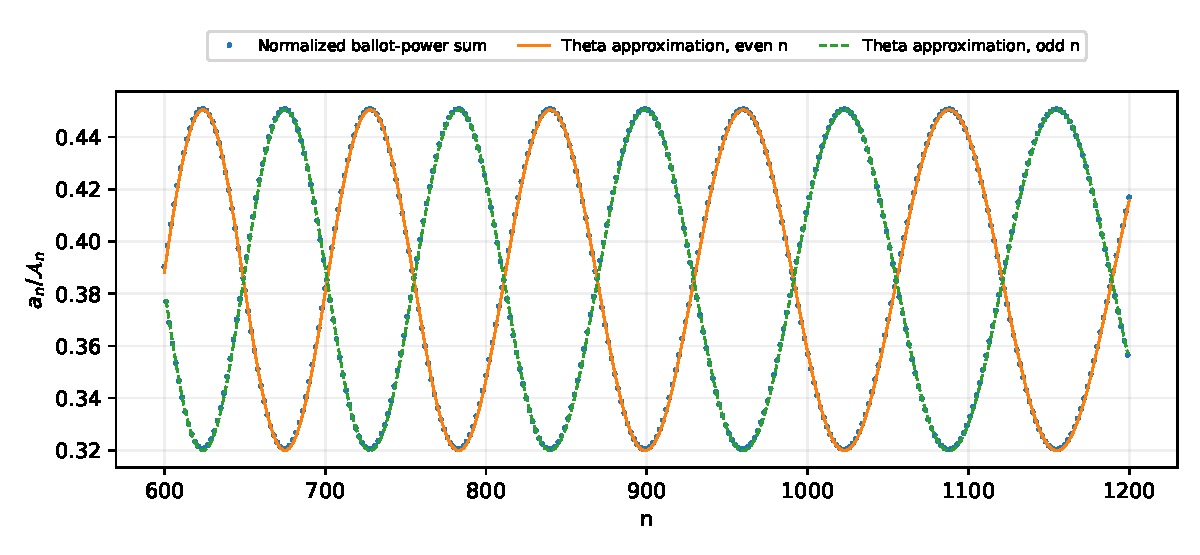
\includegraphics[width=0.98\textwidth]{figures/oscillation.pdf}
\caption{The normalized diagonal sequence and its leading approximation.
Connecting the even and odd indices separately reveals the two smooth
parity strands. The index-dependent widening of an oscillation is
consistent with the square-root phase. Plotting computations use a
localized log-Gamma sum; the full-sum tests are reported separately.}
\label{tbs:fig:oscillation}
\end{figure}

\subsection{Exponential corrections, near-square transitions, and inverses}
The first exponential sector was checked using exact integers for
$a_n$, $b_n$, and $n!$. For $n=20,30,40,60,80,100$, the ratio of the
exact relative correction to
$\sqrt{\pi\ee}\,n^3 2^{-n}/(4\sqrt2)$ ranges from approximately
$0.99969$ to $1.01631$. Its order-$1/n$ phase dependence, rather than a
single monotone convergence curve, is predicted by
\eqref{tbs:eq:first-sector}. The complete values are in
\code{data/exponential\_sector.csv}.

For the second localization transition, the code evaluates full sums
at $s=8,16,32$, $d=-2,-1,0,1,2$, and
$k=\operatorname{round}(0.3s^3)$. The resulting upper-endpoint
probabilities are compared with
$(1+\exp(-1.2d))^{-1}$ in \code{data/square\_transition.csv}.
The precise choice of the parity-preserving window
$n=s^2-2+2d$ is tested rather than replaced by a nearby generic index.

The inverse computations use $L=\log a_n$ from the full endpoint sum.
They compare \eqref{tbs:eq:explicit-inverse} with a numerical root of the
order-$6$ model of matching parity. Representative signed errors are:
\begin{center}
\small
\begin{tabular}{@{}r r r@{}}
\toprule
$n$ & Explicit inverse minus $n$ & Order-$6$ model root minus $n$\\
\midrule
100 & $-9.714\cdot10^{-4}$ & $-8.609\cdot10^{-11}$\\
200 & $-3.112\cdot10^{-4}$ & $-9.096\cdot10^{-12}$\\
400 & $-9.734\cdot10^{-5}$ & $-8.535\cdot10^{-14}$\\
800 & $-2.994\cdot10^{-5}$ & $-2.588\cdot10^{-14}$\\
1200 & $-1.506\cdot10^{-5}$ & $-4.543\cdot10^{-15}$\\
\bottomrule
\end{tabular}
\end{center}
These measurements illustrate the extra factor of order $1/n$ gained
when a logarithmic approximation is inverted. They do not provide a
certified least threshold for the big-$\OO$ statements.

\subsection{Reproducing the files}
From the extracted archive, run
\begin{verbatim}
python -m pip install -r requirements.txt
python code/verify.py --all
pdflatex -interaction=nonstopmode -halt-on-error article.tex
pdflatex -interaction=nonstopmode -halt-on-error article.tex
pdflatex -interaction=nonstopmode -halt-on-error article.tex
\end{verbatim}
The code uses Python 3.10 or newer with SymPy, mpmath, and matplotlib.
The verification itself does not require network access; the OEIS values
used in exact comparisons are embedded with their provenance. The first
command is only for installing missing dependencies. Alternatively,
\code{build.sh} compiles the article when the dependencies are already
installed. The archive includes the figures used by the TeX source,
raw CSV tables, generated coefficient polynomials, and the actual
verification-status JSON.

No Lean file is included, because no formal proof was compiled for this
report. No interval certificate is implied by a large working precision.
The existing repo was inspected but not modified.

\emph{[Write note, batch 73O1.]} In the collection the requirements file
is \code{data/requirements.txt} and the build script is
\code{code/build.sh}. The script changes into its own directory before
calling \code{code/verify.py}, so it runs only in the delivered layout.
\code{code/verify.py --all} rewrites \code{data/} and \code{figures/} in
place, so the shipped records should be regenerated on a copy; the README
gives commands that do this.

\section{Further research questions and concrete next steps}\label{tbs:sec:research}

The following questions are distinguished from the theorems already
proved. They suggest a program extending the results rather than
merely repeating the missing-constant question.

\begin{enumerate}[leftmargin=*,label=\textbf{Q\arabic*.}]
\item \textbf{Effective remainders and certified OEIS additions.}
Make the constants in \eqref{tbs:eq:local-remainder} explicit at orders
$J=0,2,4$, and combine them with interval evaluation of the theta sums.
This would yield rigorous numerical enclosures for every sufficiently
large index, an explicit log-convexity threshold, and certified threshold
inversion. A finite exact check could then bridge the remaining initial
range. The global trigamma estimate and the explicit two-site bound
already provide useful non-asymptotic ingredients.

\item \textbf{Global strict log-convexity.}
Do $a_{n-1}a_{n+1}>a_n^2$ and $b_{n-1}b_{n+1}>b_n^2$ hold at every
$n\ge1$? The limiting Tur\'an gap proves eventual strictness, but does
not settle the finite range without explicit error constants. A direct
injection, total-positivity argument, or inequality linking adjacent
ballot rows might prove the global statement without enumeration.

\item \textbf{Uniform secondary transition expansions.}
The exact two-site formula resolves the entire supercritical regime,
and Corollary~\ref{tbs:cor:logistic} resolves bounded square-window shifts.
Develop uniform expansions when the integer displacement $d$ grows with
$s$, or when $k/s^3$ tends to zero or infinity simultaneously with $d$.
The controlling variable is the exact $k\log\rho$, so a meaningful goal
is a hierarchy of elementary scaled formulas with explicit error domains,
not replacing an exact expression by an uncontrolled Taylor truncation.

\item \textbf{Optimal truncation and additional exponential scales.}
The all-orders diagonal expansion is not an optimal-truncation theorem.
Determine the large-order growth of the polynomials and theta-derivative
coefficients, and whether a rigorously optimally truncated remainder can
be decomposed into further exponential contributions. This problem is
separate from the rigorously established tuple--multiset sectors; it
should not be called resurgence without additional analysis.

\item \textbf{A growing number of multiset sectors.}
Theorem~\ref{tbs:thm:sectors} keeps $Q$ fixed. Find useful ranges of
$Q=Q(n)$ with uniform coefficient and remainder control, and study
multisets whose size differs from the path length. The elementary
symmetric coefficients of $0,\ldots,n-1$ and the ratio $k/m$ then
interact in a two-parameter problem. An exact rising-factorial bridge
remains available, but uniform asymptotic division requires new estimates.

\item \textbf{A reusable lattice-peak theorem for other path models.}
Formulate sufficient hypotheses on a positive triangular array
$C_{n,h}$ for a high-power sum to have a phase-dependent theta expansion.
The proof here suggests the required data: a uniformly concave local
logarithm, a growing interior peak, a fixed endpoint lattice, derivative
expansions, and global tail domination. Apply such a theorem to weighted
meanders and finite-step walks, then to multidimensional endpoint
lattices where theta functions are associated with quadratic forms.
This is the clearest route from the present OEIS case to a broad tool.

\emph{[Write note, batch 77P2, 2 October 2026.]} The collection's report
\code{a380274-\allowbreak mahonian-\allowbreak growing-\allowbreak powers}, in the same directory as this
one (batch~77, manuscript~55), proves one more instance of the phenomenon
for another positive triangular array, the Mahonian numbers $M_n(k)$
(permutations of $n$ with $k$ inversions; OEIS A380274, A380275 are
$\sum_k M_n(k)^3$ and $\sum_k M_n(k)^4$). With $V_n$ the inversion
variance and $C_n$ the central coefficient, its theorem ``Complete
growing-power leading behavior'' gives
$\sum_k M_n(k)^{r}/C_n^{r}\sim\Theta_\delta(r/V_n)$ for every $r=r_n\to\infty$,
a discrete Gaussian theta function whose lattice shift
$\delta\in\{0,\tfrac12\}$ is fixed by $n\bmod 4$; there is no varying
phase as in Theorem~\ref{tbs:thm:critical}. Its proof uses Fourier
estimates and log-concavity of the Mahonian row, not hypotheses of the
kind asked for here. It is an instance, not the general theorem, and this
question stays open. That report's section ``Literature boundary and
interpretation'' says the same in a note and gives the dictionary between
the two theta normalizations: its $Z_\delta(q)=\sum_{x\in\Z+\delta}\ee^{-qx^2/2}$
equals $\Theta_{q/8}(\delta)$ in the notation of \eqref{tbs:eq:theta}, and its
$\Theta_\delta(q)=\ee^{q\delta^2/2}Z_\delta(q)$; its subscript $\delta$ is a
lattice shift, the subscript $\tau$ here a scale. Neither manuscript cites
the other.

\emph{[Write note, batch 98D, 5 October 2026.]} The question is answered
in a sufficient-hypothesis form by Part~II. Its
Theorem~\ref{tbs:lpt:thm:transfer} gives the theta limit for a general
positive array under a local quadratic law, a Gaussian majorant and
interior completeness, with arbitrary drifting phase;
Theorem~\ref{tbs:lpt:thm:allorders} gives every fixed order through a
Bell-polynomial recurrence, and Theorem~\ref{tbs:lpt:thm:multi} the
multidimensional version with a quadratic-form theta function. This
report's critical regime satisfies the hypotheses
(Proposition~\ref{tbs:lpt:prop:ballot}), and so does the Mahonian
report's critical window once the Gaussian majorant is weakened to an
exponential one, which log-concavity supplies
(Proposition~\ref{tbs:lpt:prop:mahonian}). The sentence above that ``this
question stays open'' is therefore superseded. Still open are a
characterization, degenerate, boundary and multiple peaks, and concrete
weighted-meander or multidimensional applications
(Section~\ref{tbs:lpt:sec:questions}). In Part~II's notation the
Mahonian $Z_\delta(q)$ and this report's $\Theta_{q/8}(\delta)$ are both
$\vartheta(q,\delta)$ (equation~\eqref{tbs:lpt:eq:dictionary}).

\item \textbf{Joint phase laws and higher discrete differences.}
Determine effective joint laws of several neighboring normalized terms,
and use them to analyze higher logarithmic differences or Jensen
polynomials. Adjacent terms undergo a half-period shift rather than an
independent random phase. The second difference is positive because its
explicit theta quotient has a gap; analogous sign or hyperbolicity
claims at higher orders require separate proofs.

\item \textbf{Sharper averaging errors.}
The elementary discrepancy proof gives $\OO(\sqrt N)$ counting error.
For smooth periodic test functions, exploit the square-root phase,
parity cancellation, and vanishing odd corrections to seek sharper
Ces\`aro expansions. Such expansions may contain boundary-phase terms
rather than a universal constant at the next order. An unsmoothed
interval discrepancy and a smooth weighted average need not have the
same best error term.

\item \textbf{The separate arithmetic conjecture.}
The OEIS records Bala's conjecture
$a_{2p-1}\equiv1\pmod{p^3}$ for primes $p\ge5$ \cite{oeisa}.
Nothing in the present asymptotic proof establishes it. The exact shifted
ballot formula gives a possible starting point for a prime-adic analysis,
but real asymptotic errors, even exponentially small relative errors,
have no direct force modulo $p^3$. A future arithmetic report should
maintain that distinction explicitly.

\item \textbf{Formalization with a visible theorem boundary.}
Start with exact path semantics, reflection, shifted binomial identities,
the adjacent-entry ratio, and the rising-factorial bridge. Next formalize
the discrete two-site tail bound, which avoids Stirling theory. Only then
build the analytic layer: gamma remainders, summable Gaussian bounds,
phase-uniform termwise expansion, and theta identities. This staged plan
could produce useful Lean theorems before the entire analytic result is
available, without labeling the unformalized remainder as checked.
\end{enumerate}

\section{Conclusion}
The central obstacle was not the exponential scale of the counts. That
scale was already visible in the OEIS. The missing information lay in
the interaction between a moving ballot peak and an endpoint lattice
that remains coarse after taking a power proportional to the row index.
Keeping that lattice produces an explicit theta multiplier, not a
constant, and supports a complete algebraic expansion with uniform
remainders.

The same analysis produces exact fluctuation envelopes and phase laws,
strict eventual log-convexity, and stable branchwise inverse formulas.
An exact adjacent-entry ratio further identifies the mode and controls
all supercritical powers, including a second near-square transition.
Finally, an exact symmetric-polynomial identity places the multiset
sequence into a hierarchy of exponentially small corrections to the
ordered-tuple sequence. Together these results turn a recorded
nonconvergence phenomenon into a coherent analytic and combinatorial
structure, while leaving the distinct arithmetic and formalization
questions clearly identified.

\part{A lattice-peak transfer theorem for growing power sums}
\label{tbs:lpt:part}

\section{Provenance, scope and notation of Part II}\label{tbs:lpt:sec:front}

\emph{[Write note, batch 98D, 5 October 2026.]} Part~II was added in the
write of batch~98D. It prints one manuscript, which answers question~Q6
of Part~I (Section~\ref{tbs:sec:research}) in a sufficient-hypothesis
form: a general theorem of which Part~I's critical theta regime
(Theorem~\ref{tbs:thm:critical}) and the Mahonian report's critical
window are instances.

\subsection{Provenance}\label{tbs:lpt:sec:provenance}
The source is the archive
\nolinkurl{ProveIt_OEIS_Lattice_Peak_Transfer_2026-10-05.zip}, a late
arrival of batch~98 of ProveIt's incoming-reports intake (its twelfth
manuscript, the only one of placement 98D), which arrived in commit
\code{1ec443bc4} and was placed in this report by commit
\code{3b9458b31}. It holds only the article
\nolinkurl{ProveIt_OEIS_Lattice_Peak_Transfer.tex} (641 lines) and its
14-page PDF, titled \emph{A Lattice-Peak Transfer Theorem for Growing
Power Sums}, with the subtitles ``Phase-dependent theta asymptotics,
all-orders corrections, multidimensional peaks, and inverse transfer''
and ``Applications to the OEIS ballot-power and Mahonian-power
families''. It is dated 5 October 2026; its author line is ``Research
report for the ProveIt project''. Whether it was prepared with an AI
assistant is not stated. It names no pinned commit: its source audit
(Appendix~\ref{tbs:lpt:app:audit}) says the repository facts were
``checked against the ProveIt default branch on 5 October 2026'', and it
knows the batch-77P2 note of 2 October 2026 at the end of question~Q6
(commit \code{67d54b7ac}). Both reports it cites, this one and
\nolinkurl{a380274-mahonian-growing-powers}, were unchanged between that
commit and the placement. No code, data, README or checksum list was
delivered, so nothing was staged; the article and its PDF survive in the
arrival commit. Part~II is unrefereed, and nothing in it is formalized.

\subsection{What the write changed}\label{tbs:lpt:sec:changes}
Section~$k$ of the manuscript is Section~$k+12$ here, and its
Appendices~A and~B are Appendices~\ref{tbs:lpt:app:lemmas}
and~\ref{tbs:lpt:app:audit}. Within each section every numbered statement
and equation keeps the manuscript's number after that shift (manuscript
Theorem~3.1 is Theorem~\ref{tbs:lpt:thm:transfer}, equation~(5.9) is
\eqref{tbs:lpt:eq:u3}); the write's additions follow the manuscript's
numbered items of their section. All labels carry the prefix
\code{tbs:lpt:}. Symbols that collide with Part~I or with the Mahonian
report are renamed (Table~\ref{tbs:lpt:tab:notation}); otherwise the
text is the manuscript's, with references to ``the ballot report''
turned into references to Part~I. The write added, marked
\emph{[write]}:
\begin{itemize}
\item the correction of a false identity of the manuscript's Section~5.1
 (Remark~\ref{tbs:lpt:rem:u3}, with a counterexample);
\item the completion of two proofs: the theta-side tail in the all-orders
 theorem (Theorem~\ref{tbs:lpt:thm:allorders}) and the existence and
 localisation step of the inverse theorem
 (Theorem~\ref{tbs:lpt:thm:inverse}); a definition of ``local
 completeness'' in Theorem~\ref{tbs:lpt:thm:multi}; a proof of
 Corollary~\ref{tbs:lpt:cor:no-constant};
\item an exponential-majorant form of the transfer theorem
 (Theorem~\ref{tbs:lpt:thm:exp-majorant}) and a log-concavity criterion
 for it (Proposition~\ref{tbs:lpt:prop:logconcave}), with which the
 Mahonian critical window is proved to fit the hypotheses
 (Proposition~\ref{tbs:lpt:prop:mahonian}); the manuscript only predicted
 this;
\item a verification that the ballot array satisfies the hypotheses
 (Proposition~\ref{tbs:lpt:prop:ballot}), the correction of the
 manuscript's claim that Part~I's all-orders coefficients are
 ``precisely'' its own (Remark~\ref{tbs:lpt:rem:precisely}), the
 normalization of the cluster set \eqref{tbs:lpt:eq:a357825-cluster}, and
 the branchwise application of the inverse theorem to Part~I's models
 (Remark~\ref{tbs:lpt:rem:ballot-inverse});
\item the section of further questions (Section~\ref{tbs:lpt:sec:questions}),
 which keeps the manuscript's R1--R12 and adds every claim of the
 manuscript that is not proved.
\end{itemize}
Under Vladimir's standing rule of 4 October 2026 on unproved and wrong
claims: one identity is refuted with a counterexample
(Remark~\ref{tbs:lpt:rem:u3}); one identification is shown overstated
(Remark~\ref{tbs:lpt:rem:precisely}); the unproved claims are listed in
Section~\ref{tbs:lpt:sec:questions}, items F1--F7.

\subsection{Notation}\label{tbs:lpt:sec:notation}
Three theta functions appear in this report and its neighbour, and they
are normalized differently. Part~II writes
\begin{equation}\label{tbs:lpt:eq:dictionary}
 \vartheta(q,\delta)=\sum_{j\in\Z}\ee^{-\frac q2(j-\delta)^2}
 =\Theta_{q/8}(\delta)
 =Z_\delta(q)
 =\ee^{-q\delta^2/2}\,\Theta^{\mathrm{mgp}}_\delta(q),
\end{equation}
where $\Theta_\tau(\alpha)$ is Part~I's \eqref{tbs:eq:theta}, whose
subscript is a scale, and $Z_\delta(q)$ and
$\Theta^{\mathrm{mgp}}_\delta(q)=\ee^{q\delta^2/2}Z_\delta(q)$ are the
Mahonian report's (its equation \code{mgp:eq:theta}), whose subscript is a
lattice shift \cite{lptMahonian}. In particular Part~I's $\Theta(\alpha)=\Theta_1(\alpha)$ is
$\vartheta(8,\alpha)$, not $\vartheta(1,\alpha)$, and the Mahonian
$\Theta^{\mathrm{mgp}}_\delta(q)$ equals $\vartheta(q,\delta)$ only at
$\delta=0$. The identities \eqref{tbs:lpt:eq:dictionary} were checked
numerically to 18 digits at three points.

\begin{longtable}{@{}>{\raggedright}p{0.2\textwidth}>{\raggedright}p{0.27\textwidth}>{\raggedright}p{0.14\textwidth}p{0.3\textwidth}@{}}
\caption{Symbols of Part~II that differ from the manuscript or collide
with Part~I or the Mahonian report (mgp).}\label{tbs:lpt:tab:notation}\\
\toprule
Part~II & Meaning & Manuscript & Elsewhere\\
\midrule\endfirsthead
\toprule
Part~II & Meaning & Manuscript & Elsewhere\\
\midrule\endhead
$\vartheta(q,\delta)$ & translated theta series \eqref{tbs:lpt:eq:theta} & $\Theta(q,\delta)$ & Part~I $\Theta_\tau$, $\Theta$; mgp $Z_\delta$, $\Theta_\delta$; see \eqref{tbs:lpt:eq:dictionary}\\
$\vartheta_{\mathbf Q}(\delta)$, $\mathbf Q_n$, $\mathbf Q$ & quadratic-form theta series and forms & $\Theta_Q$, $Q_n$, $Q$ & Part~I $Q$: number of multiset sectors (Theorem~\ref{tbs:thm:sectors})\\
$Q_m(u;q)$ & Bell polynomials \eqref{tbs:lpt:eq:bell-rec} & $Q_m$ & as above\\
$\mathcal T_m(q,\delta)$ & all-orders coefficients & same & Part~I $T_\pm$: Tur\'an constants\\
$L_n=\xi_n+d_n\Z$, $\nu_n$ & lattice, offset, integer part & $\Lambda_n=a_n+d_n\Z$, $m_n$ & Part~I $a_n$ (A357825), $\Lambda(\alpha)$, $m=n+1$\\
$L_n=\boldsymbol\xi_n+\mathbf D_n\Z^d$ & $d$-dimensional lattice & $b_n+D_n\Z^d$ & Part~I $b_n$ (A357871), $D_j(u)$\\
$\Omega_n$ & carrier amplitude & $A_n$, $A_n^{(0)}$ & Part~I $A_\ell(x)$, $\Acal_n$\\
$t_n$ & small parameter of the all-orders theorem & $\eps_n$ & Part~I $\eps_n=m\bmod2$; Part~I $t=m^{-1/2}$ is $t_n$ in Section~\ref{tbs:lpt:sec:ballot}\\
$B_*$, $c_*$ & majorant constants of (H2) & $B$, $c$ & Part~I $B(n,h)$, $c$ in \eqref{tbs:eq:g}, $C,c$ in Lemma~\ref{tbs:lem:gaussian}\\
$\mathcal D$ & set of phase accumulation points & $D$ & Part~I $D_j(u)$\\
$\operatorname{gap}(\delta)$ & squared-distance gap in Proposition~\ref{tbs:lpt:prop:theta-regimes} & $\gamma(\delta)$ & ---\\
$\omega_{n,j}$, $\gamma_{n,j}$ & powered summand and Gaussian in proofs & $T_{n,j}$, $G_{n,j}$ & Part~I $T_\pm$, $g$\\
$\tilde H(x)$ & non-theta part of $H$ in Theorem~\ref{tbs:lpt:thm:inverse} & $h_0(x)$ & Part~I $h$: height\\
$I_n(k)$, $z$ & Mahonian numbers, $q$-factorial variable & $M_n(j)$, $q$ & Part~I $M_p$, $M_{p,\tau}$: moments; mgp $M_n(k)$\\
$\sigma_n^2$ (Mahonian) & inversion variance & $V_n$ & Part~I $V_m$; mgp $V_n$\\
$r_n$ & the growing power & $r$ & Part~I: the power is $k$ and $r=h+1$; Section~\ref{tbs:lpt:sec:ballot} uses Part~I's letters\\
$\sigma_n$ & curvature scale & same & Part~I $\sigma\in\{0,1\}$: parity branch (Section~\ref{tbs:sec:inverse})\\
$R$, $R_n$; $R(x)$ & window radii; remainder in \eqref{tbs:lpt:eq:logF} & same & Part~I $R_j(u)$: correction polynomials\\
$K=[q_-,q_+]$ & compact scale window & same & Part~I $K_n$\\
$C_{n,x}$; $C_n$ & array entry; mgp's central coefficient & same & Part~I $C_\pm$, $C$\\
$\delta_n\in[-\frac12,\frac12)$ & lattice phase & same & mgp $\delta=\mu-\lfloor\mu\rfloor\in\{0,\frac12\}$; $\vartheta$ is even and $1$-periodic in $\delta$, so the two conventions give the same values\\
\bottomrule
\end{longtable}

\section{Problem, scope, and relation to the OEIS reports}\label{tbs:lpt:sec:problem}

Let $C_{n,k}>0$ be a positive triangular array, with $k$ belonging to a
one-dimensional lattice that may translate with $n$. For an exponent
$r=r_n>0$ consider
\begin{equation}\label{tbs:lpt:eq:power-sum}
 S_n(r)=\sum_k C_{n,k}^{\,r}.
\end{equation}
When $r$ is fixed and the row has a central-limit shape, the usual
local-limit/Riemann-sum heuristic gives a Gaussian integral. When $r$
grows, raising the row to the $r$th power narrows its effective width by
$r^{-1/2}$. The transition occurs when that width becomes comparable to
the lattice spacing. At that point a Riemann integral is no longer the
correct leading object: the individual lattice sites survive, and the
answer is a theta sum.

This mechanism is visible in two existing ProveIt reports. The report on
the ballot array $S_{n,k}=\sum_h B(n,h)^k$ (Part~I) proves a critical
theta regime for $k\asymp n$ and asks, as its Question Q6, for ``a
reusable lattice-peak theorem for other path models.'' A later report on
Mahonian power sums proves the same type of transition when the power is
comparable to the inversion variance, but explicitly records itself as an
instance rather than a solution of Q6. The public OEIS entry A357825
records the diagonal ballot power sum and a nonconvergent normalized
ratio, while A380275 records fixed-power Mahonian asymptotics; Wang's 2026
preprint proves the fixed-real-power Mahonian expansion but does not claim
uniformity in a growing power \cite{oeisa,lptA380275,lptWang}.

The present report addresses precisely the missing abstraction. It
deliberately does \emph{not} try to supersede general discrete Laplace
theory. Recent work of Helton, Hughes and Schlosser \cite{discretelaplace}
treats discrete Laplace asymptotics in the regime where a lattice becomes
fine in the natural Laplace scale. Our focus is the complementary
critical regime in which the rescaled lattice has a nonzero limiting
mesh, so the lattice survives as a theta multiplier.

\subsection*{Main contributions}
The new statements proved here are:
\begin{enumerate}[label=(\roman*)]
\item a one-dimensional lattice-peak transfer theorem with arbitrary
 drifting phase and uniformity on compact critical windows;
\item a stable version for subsequences with only compactness, yielding
 the complete set of theta cluster values;
\item an all-orders theorem whose coefficients are generated by a
 universal Bell-polynomial recurrence and can be written through theta
 derivatives;
\item a multidimensional version with a positive-definite Hessian and a
 translated lattice theta function;
\item an inverse-transfer theorem showing exactly how the theta factor
 perturbs a smooth inverse;
\item a dictionary recovering the leading critical theorems of the ballot
 and Mahonian OEIS reports as instances.
\end{enumerate}
The theorem is sufficient, not necessary: many arrays will satisfy weaker
hypotheses. Its value is that each hypothesis is checkable by standard
local asymptotic and tail tools.

\emph{[write]} For item~(vi): the ballot array satisfies the hypotheses
(Proposition~\ref{tbs:lpt:prop:ballot}); the Mahonian array satisfies
them with the Gaussian majorant (H2) replaced by the exponential majorant
(H2e) of Theorem~\ref{tbs:lpt:thm:exp-majorant}
(Proposition~\ref{tbs:lpt:prop:mahonian}). The manuscript's abstract says
that both ``fit the hypotheses''; its Section~9 only predicts it for the
Mahonian array.

\section{The lattice-peak normalization}\label{tbs:lpt:sec:normalization}

\begin{definition}[Moving lattice and phase]\label{tbs:lpt:def:lattice}
For each $n$, let
\[
 L_n=\xi_n+d_n\Z,\qquad d_n>0,
\]
and let $x_n\in\R$ be a distinguished continuous peak location. Choose
$\delta_n\in[-1/2,1/2)$ so that
\begin{equation}\label{tbs:lpt:eq:phase}
 x_n=\xi_n+d_n(\nu_n+\delta_n)
\end{equation}
for some $\nu_n\in\Z$. Thus the lattice sites near the peak are
\[
 x_{n,j}=x_n+d_n(j-\delta_n),\qquad j\in\Z.
\]
The number $\delta_n$ is the \emph{lattice phase} of the continuous peak.
\end{definition}

Let $\Omega_n>0$ be a continuous carrier amplitude and
$\sigma_n\to\infty$ the curvature scale. We write
\begin{equation}\label{tbs:lpt:eq:qdef}
 q_n=\frac{r_n d_n^2}{\sigma_n^2}.
\end{equation}
The critical window is $q_n\asymp1$. The basic translated theta function
is
\begin{equation}\label{tbs:lpt:eq:theta}
 \vartheta(q,\delta)=\sum_{j\in\Z}
 \exp\!\left[-\frac q2(j-\delta)^2\right],
 \qquad q>0,
\end{equation}
which is $1$-periodic and even in $\delta$ modulo integers.

\begin{definition}[Critical lattice-peak hypotheses]\label{tbs:lpt:def:hyp}
Fix a compact interval $K=[q_-,q_+]\subset(0,\infty)$. A family $C_{n,k}$
satisfies the critical lattice-peak hypotheses on $K$ if, whenever
$r_n>0$ is chosen so that $q_n\in K$, the following hold.
\begin{enumerate}[label=\textup{(H\arabic*)}]
\item \textbf{Local quadratic law.} For every fixed $R>0$,
\begin{equation}\label{tbs:lpt:eq:localquad}
 \sup_{|j-\delta_n|\le R}
 \left|r_n\log\frac{C_{n,x_{n,j}}}{\Omega_n}
 +\frac{q_n}{2}(j-\delta_n)^2\right|\longrightarrow0.
\end{equation}
Here $C_{n,x}$ denotes the row entry at the lattice site $x$.
\item \textbf{Uniform Gaussian domination.} There are constants
$B_*,c_*>0$, independent of $n$ and of $q_n\in K$, such that for every
admissible lattice site,
\begin{equation}\label{tbs:lpt:eq:gaussdom}
 \left(\frac{C_{n,x_{n,j}}}{\Omega_n}\right)^{r_n}
 \le B_*\exp[-c_*(j-\delta_n)^2].
\end{equation}
\item \textbf{Interior completeness.} For every fixed $R$, all sites with
$|j-\delta_n|\le R$ are admissible for sufficiently large $n$.
\end{enumerate}
\end{definition}

The hypotheses separate the proof into the two ingredients that
repeatedly appear in concrete OEIS analyses: a local
Taylor/Stirling/Edgeworth expansion and a global log-concavity or Fourier
tail estimate. Notice that no probabilistic interpretation is required.

\section{The critical theta transfer theorem}\label{tbs:lpt:sec:transfer}

\begin{theorem}[One-dimensional lattice-peak transfer]\label{tbs:lpt:thm:transfer}
Assume the hypotheses of Definition~\ref{tbs:lpt:def:hyp}. Then,
uniformly for all exponent choices with $q_n\in K$,
\begin{equation}\label{tbs:lpt:eq:maintransfer}
 \frac{S_n(r_n)}{\Omega_n^{r_n}}
 =\vartheta(q_n,\delta_n)+o(1).
\end{equation}
More generally, if the local law has a uniform additive error
$\eta_n(R)$ on $|j-\delta_n|\le R$, then for every fixed $R$
\begin{align}\label{tbs:lpt:eq:explicitbound}
 \left|\frac{S_n(r_n)}{\Omega_n^{r_n}}-\vartheta(q_n,\delta_n)\right|
 &\le \left(\ee^{\eta_n(R)}-1\right)
       \sum_{|j-\delta_n|\le R}\ee^{-q_n(j-\delta_n)^2/2}\\
 &\quad +B_*\sum_{|j-\delta_n|>R}\ee^{-c_*(j-\delta_n)^2}
       +\sum_{|j-\delta_n|>R}\ee^{-q_-(j-\delta_n)^2/2},\notag
\end{align}
for all sufficiently large $n$.
\end{theorem}

\begin{proof}
Write
\[
 \omega_{n,j}=\left(C_{n,x_{n,j}}/\Omega_n\right)^{r_n},\qquad
 \gamma_{n,j}=\exp[-q_n(j-\delta_n)^2/2].
\]
Fix $R$. By interior completeness all lattice sites in the finite window
$|j-\delta_n|\le R$ occur in the row for large $n$. The local quadratic
law gives
\[
 \omega_{n,j}=\gamma_{n,j}\ee^{e_{n,j}},\qquad |e_{n,j}|\le\eta_n(R),
\]
there, proving the first term in \eqref{tbs:lpt:eq:explicitbound}.
Outside the window, hypothesis (H2) bounds the actual row tail by the
second term, while $q_n\ge q_-$ bounds the omitted theta tail by the
third. The two Gaussian tails tend to zero uniformly as $R\to\infty$, and
then $\eta_n(R)\to0$ for fixed $R$. This proves
\eqref{tbs:lpt:eq:maintransfer} by the standard ``first $n$, then $R$''
argument. Every estimate is uniform in $q_n\in K$ and in the phase
because translating a unit lattice does not change the elementary
Gaussian tail bound by more than an absolute constant.
\end{proof}

\begin{corollary}[Critical subsequential limits and phase law]\label{tbs:lpt:cor:clusters}
Suppose $q_n\to q\in(0,\infty)$. If $\delta_{n_j}\to\delta$ along a
subsequence, then
\begin{equation}\label{tbs:lpt:eq:subseq}
 \frac{S_{n_j}(r_{n_j})}{\Omega_{n_j}^{r_{n_j}}}
 \longrightarrow\vartheta(q,\delta).
\end{equation}
Consequently, if the set of phase accumulation points is
$\mathcal D\subset\R/\Z$, the set of accumulation points of the
normalized power sum is exactly
\begin{equation}\label{tbs:lpt:eq:cluster-set}
 \vartheta(q,\mathcal D)=\{\vartheta(q,\delta):\delta\in\mathcal D\}.
\end{equation}
If the phases are dense modulo $1$, the cluster set is the full compact
interval
\[
 [\min_\delta\vartheta(q,\delta),\max_\delta\vartheta(q,\delta)].
\]
\end{corollary}

\begin{proof}
The theta series and all its phase derivatives converge locally uniformly
for $q>0$, so $\vartheta(q_n,\delta_n)\to\vartheta(q,\delta)$ on any
convergent phase subsequence. Theorem~\ref{tbs:lpt:thm:transfer} supplies
the same limit for the normalized power sum. Compactness of the circle
gives the converse inclusion for cluster points. Continuity maps a
connected dense phase closure to the interval between its extrema.
\end{proof}

\begin{remark}[Why a ``constant amplitude'' can fail]\label{tbs:lpt:rem:constant}
At fixed power, a local central limit theorem often produces one Gaussian
integral and hence one constant. In the critical regime, the mesh after
peak rescaling is asymptotically nonzero. The phase $\delta_n$ is
therefore not an error term: it is part of the leading order. Replacing
$\vartheta(q,\delta_n)$ by its phase average is generally false pointwise,
even when it is correct after Ces\`aro averaging under an
equidistribution hypothesis.
\end{remark}

\emph{[write]} The proof of Theorem~\ref{tbs:lpt:thm:transfer} uses (H2)
only through the second term of \eqref{tbs:lpt:eq:explicitbound}, that is,
through a phase-uniformly summable majorant. The Gaussian form of (H2)
can therefore be weakened, and the weakened form follows from
log-concavity. The uniformity ``for all exponent choices'' in
Theorem~\ref{tbs:lpt:thm:transfer} follows from the statement for single
sequences by the usual argument: a sequence of counterexamples at
indices $n_k\to\infty$ can be completed, by any exponents with $q_n\in K$
at the other indices, to a sequence violating the single-sequence
statement.

\begin{theorem}[Exponential-majorant transfer; {[write]}]\label{tbs:lpt:thm:exp-majorant}
Let $r_n$ be a sequence of exponents with $q_n\in K$ for which (H1) and
(H3) hold, and suppose instead of (H2):
\begin{enumerate}[label=\textup{(H2e)}]
\item there are $B_*,c_*>0$ and $n_0$ such that for $n\ge n_0$ and every
 admissible site
 \begin{equation}\label{tbs:lpt:eq:expdom}
 \left(\frac{C_{n,x_{n,j}}}{\Omega_n}\right)^{r_n}
 \le B_*\exp[-c_*|j-\delta_n|].
 \end{equation}
\end{enumerate}
Then $S_n(r_n)/\Omega_n^{r_n}=\vartheta(q_n,\delta_n)+o(1)$, and
\eqref{tbs:lpt:eq:explicitbound} holds for all sufficiently large $n$ (so
that, in addition to $n\ge n_0$, the window sites are admissible in the sense
of (H3) for that $R$) with its second term
replaced by $B_*\sum_{|j-\delta_n|>R}\ee^{-c_*|j-\delta_n|}$.
\end{theorem}
\noindent\emph{Dated note (5~October 2026).} The first version of this
theorem, written at this write, said ``for $n\ge n_0$''; an independent
check found that the window sites must also be admissible, as in
Theorem~\ref{tbs:lpt:thm:transfer}'s ``sufficiently large $n$''. The
independent check (a careful reading with exact-row numerics, not a formal
verification) found the other results added at this write valid:
the log-concavity criterion, the Mahonian and ballot instances, the
theta-side tail, the completion of Theorem~19.1 and Corollary~19.2.

\begin{proof}
Repeat the proof of Theorem~\ref{tbs:lpt:thm:transfer}. The only change is
the bound for the actual row tail. For $R\ge1$ and
$\delta\in[-\frac12,\frac12)$, the sites with $|j-\delta|>R$ have
$|j|>R-\frac12$, so
\[
 \sum_{|j-\delta|>R}\ee^{-c_*|j-\delta|}
 \le2\sum_{i>R-1/2}\ee^{-c_*(i-1/2)}
 \le\frac{2\ee^{-c_*(R-1)}}{1-\ee^{-c_*}},
\]
which tends to $0$ as $R\to\infty$ uniformly in the phase. The window
term and the theta tail are unchanged.
\end{proof}

\begin{proposition}[Log-concave rows; {[write]}]\label{tbs:lpt:prop:logconcave}
Suppose that for all large $n$ the admissible sites form a set of
consecutive $j$, on which $j\mapsto C_{n,x_{n,j}}$ is positive and
log-concave:
$C_{n,x_{n,j}}^2\ge C_{n,x_{n,j-1}}C_{n,x_{n,j+1}}$. Let $r_n$ have
$q_n\in K$ and satisfy (H1) and (H3). Then (H2e) holds with
\[
 B_*=\ee^{1+3q_-},\qquad c_*=q_-.
\]
Consequently $S_n(r_n)/\Omega_n^{r_n}=\vartheta(q_n,\delta_n)+o(1)$.
\end{proposition}

\begin{proof}
Write $u_j=j-\delta_n$ and $\ell_j=\log\omega_{n,j}$, a concave sequence on
the admissible set (because $r_n>0$). By (H1) and (H3) with $R=3$, for
large $n$ every site with $|u_j|\le3$ is admissible and
$|\ell_j+q_nu_j^2/2|\le\eta$ there, where $\eta=\eta_n(3)\le\min(1,q_-/4)$.

Let $j_1$ be the least integer with $u_{j_1}\ge1$, so
$u_{j_1}\in[1,2)$ and $u_{j_1+1}\in[2,3)$. Then
\[
 \ell_{j_1+1}-\ell_{j_1}
 \le-\frac{q_n}{2}\bigl(u_{j_1+1}^2-u_{j_1}^2\bigr)+2\eta
 =-\frac{q_n}{2}(2u_{j_1}+1)+2\eta\le-\frac32q_-+2\eta\le-q_-.
\]
By concavity the increments $\ell_{j+1}-\ell_j$ do not increase, so for
every admissible $j\ge j_1+1$,
\[
 \ell_j\le\ell_{j_1+1}-q_-(j-j_1-1)\le\eta-q_-(u_j-3)
 \le1+3q_--q_-|u_j|,
\]
using $\ell_{j_1+1}\le-2q_n+\eta\le\eta$ and $u_{j_1+1}<3$. The sites
with $u_j\le-2$ are treated in the same way from the greatest $j_{-1}$
with $u_{j_{-1}}\le-1$. The remaining sites have $|u_j|<3$, where
$\ell_j\le\eta\le1\le1+3q_--q_-|u_j|$. This is \eqref{tbs:lpt:eq:expdom}.
Theorem~\ref{tbs:lpt:thm:exp-majorant} gives the conclusion.
\end{proof}

\section{Subcritical and supercritical companions}\label{tbs:lpt:sec:companions}

The critical theorem is the part needed to answer Q6, but the same
normalization clarifies both adjacent regimes.

\begin{proposition}[Theta limits at small and large $q$]\label{tbs:lpt:prop:theta-regimes}
Uniformly in $\delta\in\R$,
\begin{align}
 \vartheta(q,\delta)&=\sqrt{\frac{2\pi}{q}}\left(1+\OO\left(\ee^{-2\pi^2/q}\right)\right),&&q\downarrow0,\label{tbs:lpt:eq:theta-small}\\
 \vartheta(q,\delta)&=\sum_{j:\,|j-\delta|=\mathrm{d}(\delta)}\ee^{-q\,\mathrm{d}(\delta)^2/2}
 \left(1+\OO\left(\ee^{-q\operatorname{gap}(\delta)/2}\right)\right),&&q\to\infty,\label{tbs:lpt:eq:theta-large}
\end{align}
where $\mathrm{d}(\delta)=\dist(\delta,\Z)$ and $\operatorname{gap}(\delta)$
is the gap between the squared distance of a nearest lattice point and
the next distinct squared distance. Away from half-integer phases, the
first sum in \eqref{tbs:lpt:eq:theta-large} has one term; at half-integer
phase it has two equal terms.
\end{proposition}

\begin{proof}
Poisson summation gives
\[
 \vartheta(q,\delta)=\sqrt{\frac{2\pi}{q}}
 \sum_{m\in\Z}\ee^{-2\pi^2m^2/q}\ee^{2\pi i m\delta},
\]
from which \eqref{tbs:lpt:eq:theta-small} follows. The large-$q$
statement is direct: isolate the nearest lattice point or tied nearest
pair and bound the remaining geometric-Gaussian tail by the first omitted
squared-distance gap.
\end{proof}

\emph{[write]} The Poisson form is Part~I's \eqref{tbs:eq:poisson} at
$\tau=q/8$. In \eqref{tbs:lpt:eq:theta-large} the implied constant is
uniform in $\delta$, but the rate is not: $\operatorname{gap}(\delta)\to0$
as $\delta$ approaches a half-integer, where the bound degenerates until
the tied pair is used. (Here $\mathrm{d}(\delta)$ is the manuscript's
$d(\delta)$, renamed only to avoid the lattice span $d_n$.)

\begin{remark}[What extra hypotheses are needed outside the critical window]\label{tbs:lpt:rem:outside}
Theorem~\ref{tbs:lpt:thm:transfer} assumes $q_n$ remains in a fixed
compact subset of $(0,\infty)$. Letting $q_n\to0$ requires the local
expansion on a window whose number of lattice sites grows like
$q_n^{-1/2}$; letting $q_n\to\infty$ requires errors small enough after
multiplication by $q_n$ at the one or two nearest sites. These are
genuinely stronger demands. In applications, the subcritical side is
usually obtained from a uniform local limit theorem, while the far
supercritical side is often better handled by exact adjacent-entry
ratios, as in the ballot report (Theorem~\ref{tbs:thm:two-sites}).
\emph{[write: this remark is a heuristic; it is item F2 of
Section~\ref{tbs:lpt:sec:questions}.]}
\end{remark}

\section{An all-orders transfer theorem}\label{tbs:lpt:sec:allorders}

The leading theta theorem is only the first layer. Concrete OEIS problems
often provide a full local logarithmic expansion, and then every
coefficient can be transferred through the lattice sum.

\begin{definition}[Polynomial local expansion]\label{tbs:lpt:def:polyexp}
Let $t_n\to0$. For a fixed integer $J\ge0$, suppose that on windows
$|j-\delta_n|\le R_n$ with $R_n\to\infty$ slowly enough,
\begin{equation}\label{tbs:lpt:eq:powered-expansion}
 r_n\log\frac{C_{n,x_{n,j}}}{\Omega_n}
 =-\frac{q_n}{2}u^2+\sum_{\ell=1}^{J}t_n^\ell P_\ell(u;q_n)
 +\OO\!\left(t_n^{J+1}(1+|u|)^M\right),
 \qquad u=j-\delta_n,
\end{equation}
where each $P_\ell$ is a polynomial in $u$, with coefficients continuous
in $q\in K$, and the remainder is uniform. Assume moreover that for some
$c_*,B_*>0$ and some exponent $M'$, uniformly in $n$ and phase,
\begin{equation}\label{tbs:lpt:eq:weighted-majorant}
 \left(\frac{C_{n,x_{n,j}}}{\Omega_n}\right)^{r_n}(1+|j-\delta_n|)^{M'}
 \le B_*\ee^{-c_*(j-\delta_n)^2},
\end{equation}
and that the chosen $R_n\to\infty$ satisfies
\begin{equation}\label{tbs:lpt:eq:tail-order}
 \sum_{|j-\delta_n|>R_n}(1+|j-\delta_n|)^{M'}
       \ee^{-c_*(j-\delta_n)^2}=\OO(t_n^{J+1})
\end{equation}
uniformly in the phase. Enlarging $M'$ if necessary is harmless.
\end{definition}

Define polynomials $Q_m$ recursively by
\begin{equation}\label{tbs:lpt:eq:bell-rec}
 Q_0=1,\qquad
 mQ_m=\sum_{\ell=1}^{m}\ell P_\ell Q_{m-\ell}\quad(m\ge1).
\end{equation}
Thus
\[
 Q_1=P_1,\qquad Q_2=P_2+\frac12P_1^2,\qquad
 Q_3=P_3+P_1P_2+\frac16P_1^3.
\]

\begin{theorem}[All-orders lattice transfer]\label{tbs:lpt:thm:allorders}
Under Definition~\ref{tbs:lpt:def:polyexp}, including
\eqref{tbs:lpt:eq:weighted-majorant}--\eqref{tbs:lpt:eq:tail-order},
\begin{equation}\label{tbs:lpt:eq:allorders}
 \frac{S_n(r_n)}{\Omega_n^{r_n}}
 =\sum_{m=0}^{J}t_n^m\mathcal T_m(q_n,\delta_n)
 +\OO(t_n^{J+1}),
\end{equation}
where
\begin{equation}\label{tbs:lpt:eq:T_m}
 \mathcal T_m(q,\delta)=\sum_{j\in\Z}
 Q_m(j-\delta;q)\ee^{-q(j-\delta)^2/2}.
\end{equation}
The error is uniform for $q_n\in K$ and all phases. If the coefficients
of $P_\ell$ are smooth in $q$, then every $\mathcal T_m$ is smooth in
$(q,\delta)$.
\end{theorem}

\begin{proof}
Exponentiating \eqref{tbs:lpt:eq:powered-expansion} gives
\[
 \exp\!\left(\sum_{\ell=1}^{J}t_n^\ell P_\ell\right)
 =\sum_{m=0}^{J}t_n^m Q_m+\OO\!\left(t_n^{J+1}(1+|u|)^{M'}\right)
\]
for some $M'$, uniformly on the retained window. The coefficient
recurrence is obtained by differentiating the formal identity
$Q(t)=\exp(\sum_{\ell\ge1}t^\ell P_\ell)$ and comparing coefficients in
$tQ'(t)=Q(t)\sum_{\ell\ge1}\ell t^\ell P_\ell$. Multiplication by the
leading Gaussian and summation are justified termwise by
\eqref{tbs:lpt:eq:weighted-majorant}. The complement of the local window
is $\OO(t_n^{J+1})$ by \eqref{tbs:lpt:eq:tail-order}. Absolute and
locally uniform convergence also permits differentiation in $q$ and
$\delta$.

\emph{[write] Completion.} The last-but-one sentence bounds the actual
summands outside the window, $\omega_{n,j}\le
B_*(1+|u|)^{M'}\ee^{-c_*u^2}$; the proof also has to discard the
\emph{theta-side} tail
$\sum_{|u|>R_n}Q_m(u;q_n)\ee^{-q_nu^2/2}$, $m\le J$, which it does not
mention. Assume $M'>0$. Fix $U\ge1$ with
$M'\log(1+U)\ge\log B_*+2$, and for each $n$ a site with
$|u|\in[U,U+1]$ (one exists for every phase). For large $n$ this site
lies in the window, where \eqref{tbs:lpt:eq:powered-expansion} gives
$\omega_{n,j}\ge\ee^{-q_nu^2/2-1}$ (the polynomials $P_\ell$ have
coefficients bounded on $K$, and $t_n\to0$). Inserting this into
\eqref{tbs:lpt:eq:weighted-majorant} gives
$(c_*-q_n/2)u^2\le\log B_*+1-M'\log(1+|u|)\le-1$, hence
\[
 c_*\le\frac{q_n}2-\kappa,\qquad \kappa=(U+1)^{-2},
\]
for all large $n$. Since $|Q_m(u;q)|\le C_m(1+|u|)^{e_m}$ for $q\in K$,
\[
 \sum_{|u|>R_n}|Q_m(u;q_n)|\ee^{-q_nu^2/2}
 \le C_m\sup_{v\in\R}\Bigl[(1+|v|)^{e_m-M'}\ee^{-\kappa v^2}\Bigr]
 \sum_{|u|>R_n}(1+|u|)^{M'}\ee^{-c_*u^2},
\]
which is $\OO(t_n^{J+1})$ by \eqref{tbs:lpt:eq:tail-order}. With the two
tails discarded, the window sum of the expansion completes
\eqref{tbs:lpt:eq:allorders}. On the window, ``$R_n\to\infty$ slowly
enough'' is read as: the exponent
$\sum_\ell t_n^\ell P_\ell+\OO(t_n^{J+1}(1+|u|)^M)$ stays bounded for
$|u|\le R_n$, which is what the finite Taylor expansion of the exponential
needs. The manuscript's sentence ``Enlarging $M'$ if necessary is
harmless'' is not justified as stated: a larger $M'$ in
\eqref{tbs:lpt:eq:weighted-majorant} forces a smaller $c_*$, and
\eqref{tbs:lpt:eq:tail-order} with the smaller $c_*$ is a stronger
requirement on $R_n$. The completion above needs only $M'>0$; the case
$M'=0$ is item F6 of Section~\ref{tbs:lpt:sec:questions}.
\end{proof}

\subsection{Theta-derivative calculus}\label{tbs:lpt:sec:theta-calculus}
Polynomial-Gaussian sums in \eqref{tbs:lpt:eq:T_m} can be reduced to theta
derivatives. From
\[
 \partial_\delta\ee^{-qu^2/2}=qu\ee^{-qu^2/2},\qquad
 \partial_q\ee^{-qu^2/2}=-\frac12u^2\ee^{-qu^2/2},
\]
one obtains, for example,
\begin{align}
 \sum_j u\ee^{-qu^2/2}&=q^{-1}\partial_\delta\vartheta,\label{tbs:lpt:eq:u1}\\
 \sum_j u^2\ee^{-qu^2/2}&=-2\partial_q\vartheta,\label{tbs:lpt:eq:u2}\\
 \sum_j u^3\ee^{-qu^2/2}&=q^{-1}\partial_\delta(-2\partial_q\vartheta)
 +2q^{-2}\partial_\delta\vartheta.\label{tbs:lpt:eq:u3}
\end{align}
\emph{[write: \eqref{tbs:lpt:eq:u3} is corrected; the manuscript omits its
last term. See Remark~\ref{tbs:lpt:rem:u3}.]} Hence every coefficient in
Theorem~\ref{tbs:lpt:thm:allorders} is a finite differential operator,
with rational functions of $q$ as coefficients, applied to
$\vartheta(q,\delta)$. This is the abstract explanation for the
theta-derivative structures that appear separately in the ballot and
Mahonian calculations.

\begin{corollary}[Parity cancellation]\label{tbs:lpt:cor:parity}
Suppose $P_\ell(-u;q)=(-1)^\ell P_\ell(u;q)$. Then
$Q_m(-u;q)=(-1)^mQ_m(u;q)$. At symmetric phases $\delta\equiv0$ or
$1/2\pmod1$, every odd coefficient $\mathcal T_{2s+1}(q,\delta)$ vanishes.
\end{corollary}

\begin{proof}
The parity statement follows inductively from \eqref{tbs:lpt:eq:bell-rec}.
At integer or half-integer phase, the translated lattice is invariant
under $u\mapsto-u$, so every odd polynomial-Gaussian sum cancels term by
term.
\end{proof}

\begin{remark}[Correction of the third identity; {[write]}]\label{tbs:lpt:rem:u3}
The manuscript prints the third identity as
\begin{equation}\label{tbs:lpt:eq:u3-printed}
 \sum_j u^3\ee^{-qu^2/2}\overset{?}{=}q^{-1}\partial_\delta(-2\partial_q\vartheta),
\end{equation}
which is false. Since $u=j-\delta$,
$\partial_\delta\bigl(u^2\ee^{-qu^2/2}\bigr)=(-2u+qu^3)\ee^{-qu^2/2}$;
summing and using \eqref{tbs:lpt:eq:u1},
\[
 q^{-1}\partial_\delta(-2\partial_q\vartheta)
 =\sum_j u^3\ee^{-qu^2/2}-\frac2q\sum_ju\ee^{-qu^2/2}
 =\sum_j u^3\ee^{-qu^2/2}-2q^{-2}\partial_\delta\vartheta,
\]
which is \eqref{tbs:lpt:eq:u3}. The dropped term is not zero in general.
\emph{Counterexample:} at $q=2.7$, $\delta=0.31$ the left side of
\eqref{tbs:lpt:eq:u3-printed} is $0.0189884\ldots$
($0.01898839563097749448\ldots$), its right side is $0.0222562\ldots$
($0.02225616196228909469\ldots$), and the right side of
\eqref{tbs:lpt:eq:u3} agrees with the left to 40 digits (direct lattice
sums, the derivatives taken termwise; the printed form was also evaluated
by numerical differentiation, with the same value). The dropped term
vanishes exactly when $\partial_\delta\vartheta=0$, that is, at integer
and half-integer phases, where both sides of \eqref{tbs:lpt:eq:u3-printed}
are zero.

The general claim after the identities is true, and in a sharper form:
with $\Sigma_p=\sum_ju^p\ee^{-qu^2/2}$, the same differentiation gives
$\partial_\delta\Sigma_p=-p\Sigma_{p-1}+q\Sigma_{p+1}$, so
\begin{equation}\label{tbs:lpt:eq:moment-rec}
 \Sigma_0=\vartheta,\qquad
 \Sigma_{p+1}=q^{-1}\partial_\delta\Sigma_p+pq^{-1}\Sigma_{p-1}
 \quad(p\ge0,\ \Sigma_{-1}=0),
\end{equation}
and every $\Sigma_p$ is a polynomial in $q^{-1}$ times phase derivatives
of $\vartheta$ alone; for instance
$\Sigma_2=q^{-2}\partial_\delta^2\vartheta+q^{-1}\vartheta$ and
$\Sigma_3=q^{-3}\partial_\delta^3\vartheta+3q^{-2}\partial_\delta\vartheta$.
This is Part~I's moment recurrence \eqref{tbs:eq:momentrec} in the other
normalization: Part~I's moments are $M_{p,\tau}=2^p\Sigma_p$ at $q=8\tau$,
and at $q=8$ the two formulas give Part~I's
$M_2=\Theta''/16+\Theta/2$ and $M_3=\Theta'''/64+3\Theta'/8$
(Appendix~\ref{tbs:app:coefficients}). At the point of the counterexample
the formula for $\Sigma_3$ agrees with the direct sum to 40 digits.
\end{remark}

\section{A multidimensional lattice-peak theorem}\label{tbs:lpt:sec:multi}

Many combinatorial arrays have several coupled endpoint statistics. The
same proof survives with almost no change.

Let $L_n=\boldsymbol\xi_n+\mathbf D_n\Z^d$ be a full-rank lattice in
$\R^d$, where $\mathbf D_n\to\mathbf D$ with $\mathbf D$ invertible after
any desired normalization. Write the peak as
$x_n=\boldsymbol\xi_n+\mathbf D_n(\nu_n+\delta_n)$ with
$\delta_n\in[-1/2,1/2)^d$. Let $H_n$ be a positive-definite curvature
matrix and assume the powered local logarithm has the form
\begin{equation}\label{tbs:lpt:eq:multi-local}
 r_n\log\frac{C_{n,x_{n,j}}}{\Omega_n}
 =-\frac12(j-\delta_n)^T\mathbf Q_n(j-\delta_n)+o(1),
\end{equation}
for fixed $j$, where
\[
 \mathbf Q_n=r_n \mathbf D_n^T H_n \mathbf D_n\longrightarrow\mathbf Q>0.
\]
Define
\begin{equation}\label{tbs:lpt:eq:multi-theta}
 \vartheta_{\mathbf Q}(\delta)=\sum_{j\in\Z^d}
 \exp\!\left[-\frac12(j-\delta)^T\mathbf Q(j-\delta)\right].
\end{equation}

\begin{theorem}[Multidimensional transfer]\label{tbs:lpt:thm:multi}
Assume \eqref{tbs:lpt:eq:multi-local}, local completeness, and a uniform
summable bound
\[
 \left(C_{n,x_{n,j}}/\Omega_n\right)^{r_n}
 \le B_*\exp[-c_*\|j-\delta_n\|^2].
\]
Then
\begin{equation}\label{tbs:lpt:eq:multi-main}
 \frac{S_n(r_n)}{\Omega_n^{r_n}}
 =\vartheta_{\mathbf Q_n}(\delta_n)+o(1).
\end{equation}
If $\mathbf Q_n\to\mathbf Q$ and $\delta_n\to\delta$ along a subsequence,
the right side tends to $\vartheta_{\mathbf Q}(\delta)$.
\end{theorem}

\begin{proof}
The proof of Theorem~\ref{tbs:lpt:thm:transfer} applies verbatim with
Euclidean balls replacing intervals. The Gaussian majorant is summable on
$\Z^d$, and the family of tails is uniform because the phases remain in a
compact fundamental cube and the eigenvalues of $\mathbf Q_n$ stay
bounded above and below on a compact positive-definite set.
\end{proof}

\emph{[write]} ``Local completeness'' is not defined in the manuscript;
it is read as the $d$-dimensional form of (H3): for every fixed $R$, all
sites with $\|j-\delta_n\|\le R$ are admissible for large $n$. The local
law \eqref{tbs:lpt:eq:multi-local} is assumed for fixed $j$; since the
phases lie in a compact cube, it holds uniformly on every ball
$\|j-\delta_n\|\le R$, which is what the window step uses. The bounds on
the eigenvalues of $\mathbf Q_n$ hold for large $n$ because
$\mathbf Q_n\to\mathbf Q>0$.

\begin{remark}[Root-lattice and constrained variants]\label{tbs:lpt:rem:variants}
Nothing essential requires the lattice to be a copy of $\Z^d$. A fixed
full-rank lattice is reduced to this form by a basis matrix. If the peak
lies on an affine sublattice or a linear conservation law, one first
parametrizes that sublattice and applies the theorem in its intrinsic
dimension. Boundary peaks require half-theta or cone-theta functions and
are a separate extension. \emph{[write: the last two sentences are not
proved here; item F3 and question R3 of
Section~\ref{tbs:lpt:sec:questions}.]}
\end{remark}

\section{Inverse transfer: how theta oscillations move thresholds}\label{tbs:lpt:sec:inverse}

Growing combinatorial sequences are often inverted: given a large target
$Y$, one asks for the real or integer index at which the count reaches
$Y$. A phase-dependent multiplier produces a systematic correction.

\begin{theorem}[One-step inverse transfer]\label{tbs:lpt:thm:inverse}
Let $F(x)$ be a positive smooth interpolation of a growing sequence on an
interval $x\to\infty$, and suppose
\begin{equation}\label{tbs:lpt:eq:logF}
 \log F(x)=G(x)+H(x)+R(x),
\end{equation}
where $G'(x)>0$, $G'(x)\to\infty$ or stays bounded away from $0$,
$H(x)=O(1)$, and $R(x)=o(1)$. Let $x_0=x_0(Y)$ solve $G(x_0)=\log Y$.
Assume
\begin{equation}\label{tbs:lpt:eq:inverse-regularity}
 \frac{G''(x_0)}{G'(x_0)^2}=o(1),\qquad
 \frac{H'(x_0)}{G'(x_0)}=o(1),\qquad
 \frac{R(x_0)}{1+|H(x_0)|}=o(1).
\end{equation}
Then the solution $x=x(Y)$ of $F(x)=Y$ satisfies
\begin{equation}\label{tbs:lpt:eq:inverse-correction}
 x=x_0-\frac{H(x_0)}{G'(x_0)}
 +o\!\left(\frac{1+|H(x_0)|}{G'(x_0)}\right).
\end{equation}
If
\[
 H(x)=\log\vartheta(q(x),\delta(x))+\tilde H(x),
\]
then the theta factor contributes exactly
\begin{equation}\label{tbs:lpt:eq:theta-inverse}
 -\frac{\log\vartheta(q(x_0),\delta(x_0))}{G'(x_0)}
\end{equation}
to first order.
\end{theorem}

\begin{proof}
Put $\Delta=x-x_0$. Taylor expansion gives
\[
 0=G'(x_0)\Delta+H(x_0)+R(x_0)
 +\OO(G''(x_0)\Delta^2)+\OO(H'(x_0)\Delta)+o(|\Delta|G'(x_0)).
\]
The candidate $\Delta_0=-H(x_0)/G'(x_0)$ is $O((1+|H|)/G')$. Substituting
this scale and using \eqref{tbs:lpt:eq:inverse-regularity} shows that
every remaining term is $o(1+|H|)$. Division by $G'(x_0)$ proves
\eqref{tbs:lpt:eq:inverse-correction}.

\emph{[write] Completion.} The proof above presupposes a solution $x$
with $\Delta$ of the order of the candidate, and evaluates $G''$ and $H'$
at $x_0$ although Taylor's theorem needs them between $x_0$ and $x$. We
read $G\in C^2$, $H\in C^1$, $R$ continuous on some $[x_1,\infty)$, and
the $o(1)$ in \eqref{tbs:lpt:eq:inverse-regularity} as $Y\to\infty$.
Because $G$ is continuous and increases to $\infty$ ($G'$ is bounded
below), $x_0(Y)$ runs through every large real number, so
\eqref{tbs:lpt:eq:inverse-regularity} says $G''/G'^2\to0$ and
$H'/G'\to0$ as $x\to\infty$; and the third condition follows from
$R=o(1)$.

\emph{Existence and localisation.} Let $K_0\ge\sup_{x\ge x_1}(|H|+|R|)$,
enlarging $x_1$ if needed, and let $X=G^{-1}$. For
$s\in I=[\log Y-K_0-1,\log Y+K_0+1]$,
$\frac{\dd}{\dd s}\log G'(X(s))=G''(X(s))/G'(X(s))^2=o(1)$, so
$G'=G'(x_0)(1+o(1))$ on $X(I)$, and $X(I)$ lies within
$2(K_0+1)/G'(x_0)$ of $x_0$ for large $Y$. At $x_\pm=X(\log Y\pm(K_0+1))$,
$\log F(x_\pm)-\log Y=\pm(K_0+1)+H(x_\pm)+R(x_\pm)$ is positive at $x_+$
and negative at $x_-$, so $F=Y$ has a root between them by the
intermediate value theorem. Conversely every root $x\ge x_1$ has
$|G(x)-\log Y|=|H(x)+R(x)|\le K_0$, so it lies in $X(I)$. Uniqueness is
not claimed; the conclusion holds for every root.

\emph{Taylor step.} For a root $x$ and $\Delta=x-x_0$,
$|\Delta|\le2(K_0+1)/G'(x_0)$ and
\[
 0=G'(x_0)\Delta+\tfrac12G''(\xi)\Delta^2+H(x_0)+H'(\zeta)\Delta+R(x)
\]
with $\xi,\zeta\in X(I)$. There $G''(\xi)=o(G'(x_0)^2)$ and
$H'(\zeta)=o(G'(x_0))$, so the second, fourth and fifth terms are $o(1)$.
Hence $G'(x_0)\Delta=-H(x_0)+o(1)$, which implies
\eqref{tbs:lpt:eq:inverse-correction} (with $o(1/G'(x_0))$, the same
thing because $H$ is bounded). The last assertion follows by inserting
$H=\log\vartheta+\tilde H$.
\end{proof}

\begin{corollary}[No universal constant inverse correction under drifting phase]\label{tbs:lpt:cor:no-constant}
If $q(x)\to q_*>0$ while $\delta(x)$ has at least two accumulation points
at which $\vartheta(q_*,\delta)$ takes different values, then no
replacement of the theta term in \eqref{tbs:lpt:eq:theta-inverse} by a
single constant can be valid to the displayed order along all
subsequences.
\end{corollary}

This is useful conceptually: a nonconvergent normalized ratio is not
merely a nuisance in the forward asymptotics. It propagates into the
inverse as a deterministic phase oscillation.

\begin{proof}[Proof {[write]}]
The manuscript gives none. Let $\delta(x^{(i)}_k)\to\delta_i$ ($i=1,2$)
along $x^{(i)}_k\to\infty$, with
$\vartheta(q_*,\delta_1)\ne\vartheta(q_*,\delta_2)$, and take
$Y=\ee^{G(x^{(i)}_k)}$, so that $x_0=x^{(i)}_k$. If some constant $c$
gave $x=x_0-(c+\tilde H(x_0))/G'(x_0)+o(1/G'(x_0))$ along both
sequences, subtracting \eqref{tbs:lpt:eq:inverse-correction} would give
$\log\vartheta(q(x_0),\delta(x_0))-c=o(1)$ along both, hence
$\log\vartheta(q_*,\delta_1)=c=\log\vartheta(q_*,\delta_2)$ by continuity,
a contradiction.
\end{proof}

\emph{[write]} Theorem~\ref{tbs:lpt:thm:inverse} is the first-order,
real, bounded-perturbation analogue of the $M=1$ term of the perturbed
inversion theorem \code{p0:thm:perturbed-inversion} of the
series-and-transseries volume
\nolinkurl{Analysis/Transseries/docs/series-and-transseries/Transseries_And_Inversion/transseries_and_inversion.tex},
which is analytic and assumes a small perturbation parameter; neither
statement contains the other.

\section{Application I: high powers of ballot numbers}\label{tbs:lpt:sec:ballot}

Part~I studies
\[
 S_{n,k}=\sum_h B(n,h)^k,
\]
where $B(n,h)$ counts nonnegative $\pm1$ paths of length $n$ ending at
height $h$. It uses
\[
 m=n+1,\qquad r=h+1,
\]
so $r$ lies on a parity class with spacing $d=2$, and the continuous peak
is at $r=\sqrt m$. Its phase is
\begin{equation}\label{tbs:lpt:eq:ballot-phase}
 \alpha_n=\frac{\sqrt m-(m\bmod2)}{2},
\end{equation}
and its theta normalization is
\begin{equation}\label{tbs:lpt:eq:ballot-theta}
 \Theta_\tau(\alpha)
 =\sum_{j\in\Z}\ee^{-4\tau(j-\alpha)^2}.
\end{equation}
\emph{[write: this is Part~I's \eqref{tbs:eq:theta}; the manuscript writes
$\Theta^{\mathrm{bal}}_\tau$. In this section the power is Part~I's $k$,
and $r=h+1$.]}

Part~I proves, uniformly for $\tau=k/m$ in compact subsets of
$(0,\infty)$ (Theorem~\ref{tbs:thm:critical}),
\begin{equation}\label{tbs:lpt:eq:ballot-known}
 S_{n,k}=V_m^k\ee^{\tau/6}
 \left[\Theta_\tau(\alpha_n)+\OO(m^{-1/2})\right].
\end{equation}
This is exactly Theorem~\ref{tbs:lpt:thm:transfer}: in our convention
\[
 q=8\tau,\qquad \delta=\alpha_n,\qquad
 \Omega_n=V_m\ee^{1/(6m)}.
\]
The ballot report's local Stirling expansion verifies (H1), its global
trigamma/log-concavity estimate verifies (H2), and the peak remains
macroscopically far from the endpoints, giving (H3).
\emph{[write: verified in Proposition~\ref{tbs:lpt:prop:ballot}; the
phase $\alpha_n$ is used modulo~$1$.]}

The conceptual gain is not a new proof of
\eqref{tbs:lpt:eq:ballot-known}; that theorem is already in the
repository. The gain is that its theta factor is now identified as the
universal output of a reusable set of hypotheses. Moreover, the report's
all-orders coefficient functions
\[
 \sum_{j\in\Z}R_s(2(j-\alpha_n))\ee^{-4\tau(j-\alpha_n)^2}
\]
are precisely the $\mathcal T_s$ of Theorem~\ref{tbs:lpt:thm:allorders}
after the change of variable $u=2(j-\alpha_n)$. Its observed odd-order
cancellation at integer and half-integer phases is
Corollary~\ref{tbs:lpt:cor:parity}. \emph{[write: the ``precisely'' holds
only at first order with the dictionary above; see
Remark~\ref{tbs:lpt:rem:precisely}.]}

For the diagonal A357825, $k=n$ and hence $\tau=n/(n+1)\to1$. The leading
normalized ratio therefore has the cluster set
\begin{equation}\label{tbs:lpt:eq:a357825-cluster}
 \ee^{-5/6}\{\Theta_1(\delta):\delta\in\mathcal D\},
\end{equation}
where $\mathcal D$ is the phase cluster set of
\eqref{tbs:lpt:eq:ballot-phase}. The existing ballot report analyzes this
phase in detail; the transfer theorem explains why the same structure
must recur in any array with the same local lattice geometry.

\emph{[write] Normalization of \eqref{tbs:lpt:eq:a357825-cluster}.} The
``leading normalized ratio'' is Kotesovec's $a_n/\Acal_n$ of
\eqref{tbs:eq:normalizations-a}, not $a_n/\Omega_n^n$, which by
Corollary~\ref{tbs:lpt:cor:clusters} has the cluster set
$\{\Theta_1(\delta):\delta\in\mathcal D\}$ without the factor. The factor
comes from $\Omega_n^n/\Acal_n=(n/m)^n\ee^{n/(6m)}\to\ee^{-1}\ee^{1/6}$,
since $V_m=K_nn/m$ by \eqref{tbs:eq:V}. By
Proposition~\ref{tbs:prop:equidist} the phases are dense, so
$\mathcal D=\R/\Z$ and \eqref{tbs:lpt:eq:a357825-cluster} is the interval
$[C_-,C_+]$ of Theorem~\ref{tbs:thm:envelope}; numerically
$\ee^{-5/6}\vartheta(8,\tfrac12)=0.319866759530995726129\ldots$ and
$\ee^{-5/6}\vartheta(8,0)=0.450518194019661974351\ldots$, equal to
\eqref{tbs:eq:Cminus} and \eqref{tbs:eq:Cplus}.

\begin{proposition}[The ballot array satisfies (H1)--(H3); {[write]}]\label{tbs:lpt:prop:ballot}
Let $K=[8\tau_-,8\tau_+]$ with $0<\tau_-<\tau_+$, and let the exponent
$k=\tau m$ have $\tau\in[\tau_-,\tau_+]$. In the dictionary above
($d_n=2$, sites $r=\sqrt m+2(j-\alpha_n)$, $\sigma_n^2=m/2$), the ballot
rows satisfy (H1), (H2) and (H3) on $K$, with
$B_*=\ee^{2\tau_+(C+1)}$ and $c_*=4c\tau_-$, where $C,c$ are the
constants of Lemma~\ref{tbs:lem:gaussian}. Hence
Theorem~\ref{tbs:lpt:thm:transfer} recovers the leading term of
\eqref{tbs:lpt:eq:ballot-known}, with error $o(1)$ instead of Part~I's
$\OO(m^{-1/2})$.
\end{proposition}

\begin{proof}
(H1): the display in the proof of Theorem~\ref{tbs:thm:critical} gives,
with $u=r-\sqrt m=2(j-\alpha_n)$,
$k\log(\bcont_m(\sqrt m+u)/V_m)=\tau(\frac16-u^2)+\OO(m^{-1/2})$ on
bounded windows, uniformly in $\tau$; subtracting
$k\log\ee^{1/(6m)}=\tau/6$ leaves $-\tau u^2=-\frac q2(j-\alpha_n)^2$ up
to $\OO(m^{-1/2})$. (H2): Lemma~\ref{tbs:lem:gaussian} gives
$n\log(\bcont_m(r)/K_n)\le C-cu^2$ for $0<r\le m$ and large $n$. Since
$\Omega_n=K_n(n/m)\ee^{1/(6m)}$,
\[
 k\log\frac{\bcont_m(r)}{\Omega_n}
 =\frac{k}{n}\,n\log\frac{\bcont_m(r)}{K_n}+k\log\frac mn-\frac\tau6
 \le\frac{\tau m}{n}(C-cu^2)+\tau\,m\log\frac{m}{m-1},
\]
and $1\le m/n\le2$, $m\log\frac m{m-1}\le2$ give
$k\log(\bcont_m/\Omega_n)\le2\tau_+(C+1)-4c\tau_-(j-\alpha_n)^2$ (if
$C<0$, replace $C$ by $0$). (H3): the admissible $r$ are the integers of
parity $m$ in $(0,m]$, and the window sites
$\sqrt m+2(j-\alpha_n)$, $|j-\alpha_n|\le R$, lie in that range for
large $m$.
\end{proof}

\begin{remark}[``Precisely the $\mathcal T_s$'' holds only at first order; {[write]}]\label{tbs:lpt:rem:precisely}
With the dictionary printed above ($r_n=k=n$ on the diagonal, $q_n=8n/m$,
$\Omega_n=V_m\ee^{1/(6m)}$, $t_n=m^{-1/2}$), the polynomials of
Definition~\ref{tbs:lpt:def:polyexp} are obtained from
Lemma~\ref{tbs:lem:stirling} with $\tau=n/m=1-t^2$. Written in Part~I's
variable $u=2(j-\alpha_n)$, a series computation with Part~I's
$A_1,\dots,A_4$ gives
\[
 P_1=\frac{u^3}3+\frac{2u}3=D_1,\qquad
 P_2=-\frac{u^4}4-\frac7{60}\ne D_2=-\frac{u^4}4+u^2+\frac{13}{60},
\]
so $Q_1=R_1$ but
$Q_2=\frac{u^6}{18}-\frac{u^4}{36}+\frac{2u^2}9-\frac7{60}\ne R_2$
(compare \eqref{tbs:eq:R2}). Both expansions are valid (the second by
re-expanding Part~I's Theorem~\ref{tbs:thm:main}, not through the
all-orders theorem of this Part, whose hypotheses for the ballot rows are
still open, item~F7); they expand different normalized quantities. At $n=400$, $1600$, $6400$ the
truncation after $\mathcal T_2$ of $a_n/\Omega_n^n$ has relative errors
$-3.4\cdot10^{-6}$, $-2.1\cdot10^{-7}$, $-1.3\cdot10^{-8}$, and the
truncation after $F_2$ of $a_n/\Acal_n$ (Theorem~\ref{tbs:thm:main})
$7.9\cdot10^{-7}$, $5.0\cdot10^{-8}$, $3.2\cdot10^{-9}$, both
$\OO(m^{-3/2})$ (they actually fall like $m^{-2}$, by a factor of~16 per
step, because these $n$ all have phases near~$1/2$, where the odd
third-order terms nearly vanish); but $\mathcal T_2(q_n,\alpha_n)\approx0.108$ while
$F_2(\alpha_n)\approx1.090$ at these $n$. The identification is exact at
every order after re-choosing the dictionary: take $q=8$ fixed,
$t_n=m^{-1/2}$, and $\Omega_n$ with $\Omega_n^n=\ee^{-5/6}\Acal_n$. Then
\eqref{tbs:eq:master} reads
$n\log(\bcont_m(\sqrt m+u)/\Omega_n)=-u^2+\sum_{s\ge1}D_s(u)t^s$, so
$P_s(v)=D_s(2v)$ in the variable $v=j-\alpha_n$, the recurrence
\eqref{tbs:lpt:eq:bell-rec} becomes \eqref{tbs:eq:Rrecurrence},
$Q_s(v)=R_s(2v)$, and $\mathcal T_s(8,\alpha)=F_s(\alpha)$ of
\eqref{tbs:eq:F}. The display above the remark, with
$\ee^{-4\tau(\cdots)^2}$ and $\tau\ne1$, matches neither dictionary
beyond $s=1$.
\end{remark}

\begin{remark}[The inverse theorem on Part~I's branches; {[write]}]\label{tbs:lpt:rem:ballot-inverse}
The phase $\alpha_n$ jumps with the parity of $m$, so the integer
sequence $a_n$ has no smooth interpolation with a smooth phase, and
Theorem~\ref{tbs:lpt:thm:inverse} cannot be applied to it directly; the
manuscript does not carry out the application. On each parity branch it
applies to Part~I's smooth model $A_{\sigma,J}$ of
\eqref{tbs:eq:inverse-model}: take $G=g$ of \eqref{tbs:eq:g}, $R=0$ and
$H=\log\bigl(\ee^{-5/6}\sum_{j\le J}(x+1)^{-j/2}F_j(\alpha_\sigma(x))\bigr)$,
which is bounded because $\Theta\ge\ee^{-1}$, with $H'=\OO(x^{-1/2})$
because $\alpha_\sigma'(x)=1/(4\sqrt{x+1})$; and $g'(x)=2\lambda x+\OO(\log
x)$, $g''$ bounded. Then \eqref{tbs:lpt:eq:inverse-correction} gives
$r_{\sigma,J}(L)=x_0-H(x_0)/g'(x_0)+o(1/x_0)$ with $g(x_0)=L$, whose theta
part is $-\log\Theta(\alpha_\sigma(x_0))/g'(x_0)$, the
$\log\Theta$-part of the term $-d_0(\beta)/(2\lambda s)$ of
Theorem~\ref{tbs:thm:inverse}, which is sharper. A single statement for
the integer thresholds across both parities is item F5 of
Section~\ref{tbs:lpt:sec:questions}.
\end{remark}

\section{Application II: growing powers of Mahonian coefficients}\label{tbs:lpt:sec:mahonian}

Let $I_n(j)$ be the coefficient of $z^j$ in the $z$-factorial
\[
 [n]_z!=\prod_{m=1}^n(1+z+\cdots+z^{m-1}),
\]
and let
\[
 S_n(r)=\sum_j I_n(j)^r.
\]
The inversion statistic has mean
\[
 \mu_n=\frac{n(n-1)}4
\]
and variance
\[
 \sigma_n^2=\frac{n(n-1)(2n+5)}{72}.
\]
The lattice has unit spacing, while the center has phase
\[
 \delta_n=\mu_n-\lfloor\mu_n\rfloor\in\{0,1/2\}.
\]
A local Edgeworth expansion gives, in the central window,
\begin{equation}\label{tbs:lpt:eq:mahon-local}
 \log\frac{I_n(j)}{I_n(\lfloor\mu_n\rfloor)}
 =-\frac{(j-\mu_n)^2-\delta_n^2}{2\sigma_n^2}
 +\text{higher local terms}.
\end{equation}
Thus the critical parameter is
\[
 q_n=\frac{r_n}{\sigma_n^2}.
\]
When $q_n\to\rho\in(0,\infty)$, Theorem~\ref{tbs:lpt:thm:transfer}
predicts
\begin{equation}\label{tbs:lpt:eq:mahon-transfer}
 \frac{S_n(r_n)}{C_n^{r_n}}
 \sim \ee^{\rho\delta_n^2/2}
 \sum_{x\in\Z+\delta_n}\ee^{-\rho x^2/2},
 \qquad C_n=I_n(\lfloor\mu_n\rfloor),
\end{equation}
which is exactly the theta normalizer used in the repository's Mahonian
growing-power report.
\emph{[write: the manuscript's $M_n(j)$, $q$ and $V_n$ are renamed $I_n(j)$,
$z$ and $\sigma_n^2$ (Table~\ref{tbs:lpt:tab:notation}); the Mahonian
report writes $M_n(k)$ and $V_n$. The right side of
\eqref{tbs:lpt:eq:mahon-transfer} is that report's
$\Theta^{\mathrm{mgp}}_\delta(\rho)$; its phase convention $\{0,\frac12\}$
differs from Definition~\ref{tbs:lpt:def:lattice}'s $[-\frac12,\frac12)$
only by an integer, which changes nothing.]}

The public OEIS entry A380275 records the fourth-power sum and now cites
Wang's proof of the fixed-real-power asymptotic. Wang's preprint
explicitly keeps $r$ fixed and states no uniformity in $r$; the critical
scaling $r\asymp\sigma_n^2\asymp n^3$ is therefore a genuinely different
asymptotic regime. Canfield, Janson and Zeilberger provide classical
central and local-normal background for Mahonian statistics
\cite{lptCJZ}. The transfer theorem isolates the additional fact needed
for growing powers: after the local quadratic law is multiplied by $r_n$,
the unit lattice no longer disappears.

\subsection{A two-instance universality statement}\label{tbs:lpt:sec:two-instance}
The ballot and Mahonian rows have very different combinatorial origins
and different peak scales:
\begin{center}
\small
\begin{tabular}{@{}lll@{}}
\toprule
 & Ballot endpoints & Mahonian inversions\\
\midrule
continuous center & $\sqrt{n+1}$ (shifted variable) & $n(n-1)/4$\\
lattice span & $2$ & $1$\\
curvature scale & order $\sqrt n$ in endpoint coordinate & $\sigma_n\asymp n^{3/2}$\\
critical power & $k\asymp n$ & $r\asymp\sigma_n^2\asymp n^3$\\
phase & drifting square-root/parity phase & $0$ or $1/2$\\
leading critical object & translated theta sum & translated theta sum\\
\bottomrule
\end{tabular}
\end{center}
After normalization, both reduce to the same datum $(q,\delta)$ in
Theorem~\ref{tbs:lpt:thm:transfer}. This is the precise sense in which Q6
has a positive answer.

\emph{[write]} The manuscript's ``predicts'' is accurate: it does not
verify (H1)--(H3) for the Mahonian rows, and its abstract and
contribution~(vi) say more. The leading statement is proved below, with
(H2) weakened to (H2e). Its ingredients are the Mahonian report's own
(the cancellation-respecting profile estimate
\code{mgp:eq:profileleading} and log-concavity of the row), so the
proposition is a reorganization of that report's proof of its
critical window, not an independent second proof.

\begin{proposition}[The Mahonian critical window is an instance; {[write]}]\label{tbs:lpt:prop:mahonian}
Take $\xi_n=0$, $d_n=1$, $x_n=\mu_n$ (so $\delta_n\equiv\mu_n\pmod1$,
$\delta_n\in\{0,-\frac12\}$), $\sigma_n^2$ as above and
$\Omega_n=C_n\ee^{\delta_n^2/(2\sigma_n^2)}$. For every compact
$K\subset(0,\infty)$ and exponents with $q_n=r_n/\sigma_n^2\in K$, the
Mahonian rows satisfy (H1), (H2e) with $B_*=\ee^{1+3q_-}$, $c_*=q_-$,
and (H3). Consequently
\[
 \frac{S_n(r_n)}{C_n^{r_n}}
 =\ee^{q_n\delta_n^2/2}\vartheta(q_n,\delta_n)+o(1)
 =\Theta^{\mathrm{mgp}}_{\delta}(q_n)+o(1),
\]
uniformly for $q_n\in K$: the critical-window case of the Mahonian
report's Theorem \code{mgp:thm:main}.
\end{proposition}

\begin{proof}
The sites are $\mu_n+v$ with $v=j-\delta_n\in\Z+\delta$. In the Mahonian
report, $I_n(\mu_n+v)=n!\,f_n(v)$ with $f_n$ even, and $C_n=n!f_n(\delta)$
(for $\delta=\frac12$ by the symmetry $I_n(k)=I_n(N-k)$, $N=2\mu_n$). Its
estimate \code{mgp:eq:profileleading},
$\log(f_n(v)/f_n(\delta))=-\frac{v^2-\delta^2}{2\sigma_n^2}\{1+\OO_B(n^{-1})\}$
for $|v|\le B\sigma_n$ and $|v|\ge\delta$, gives on $|v|\le R$
\[
 r_n\log\frac{I_n(\mu_n+v)}{\Omega_n}
 =-\frac{q_n}{2}v^2+\frac{q_n}2(v^2-\delta^2)\,\OO_R(n^{-1}),
\]
whose error is at most $q_+R^2\OO_R(n^{-1})\to0$: this is (H1). The
window sites lie in the support $[0,N]$, $N=n(n-1)/2$, for large $n$,
which is (H3); every $I_n(k)$ with $0\le k\le N$ is positive. The
Mahonian report proves that the row is log-concave (its Section~3), so
Proposition~\ref{tbs:lpt:prop:logconcave} gives (H2e) and the transfer.
Finally $\Omega_n^{r_n}=C_n^{r_n}\ee^{q_n\delta_n^2/2}$, and
\eqref{tbs:lpt:eq:dictionary} converts $\ee^{q\delta^2/2}\vartheta(q,\delta)$
to $\Theta^{\mathrm{mgp}}_\delta(q)$.
\end{proof}

A numerical check on exact rows ($n=40,41,80,82$; $q_n=0.5,1,3$) found the
rows log-concave and the bound \eqref{tbs:lpt:eq:expdom} with these
constants satisfied with room (the largest ratio of a powered summand to
the bound was $0.106$), and window errors $\eta_n(3)$ from $0.36$ at
$n=40$, $q_n=3$ down to $0.020$ at $n=82$, $q_n=0.5$, decreasing like
$1/n$. Whether the Mahonian rows satisfy the Gaussian (H2) itself is
item F1 of Section~\ref{tbs:lpt:sec:questions}.

\section{A practical verification checklist for new OEIS arrays}\label{tbs:lpt:sec:checklist}

For future applications, the theorem suggests a short proof architecture.
\begin{enumerate}[label=\textbf{Step \arabic*.},leftmargin=*]
\item \textbf{Find a continuous carrier.} Extend the row locally to a
smooth function and locate its peak $x_n$. Record the lattice spacing and
phase before replacing $x_n$ by a rounded mode.
\item \textbf{Measure curvature.} Compute
$\sigma_n^2=-1/(\partial_x^2\log C_n)(x_n)$ to leading order. The
critical power is $r_n\asymp\sigma_n^2/d_n^2$.
\item \textbf{Expand the powered logarithm, not merely the row.} The
right error criterion is $r_n$ times the local logarithmic error. An
error negligible for fixed powers may be leading at critical powers.
\item \textbf{Prove a global summable majorant.} Log-concavity, an exact
adjacent ratio, a characteristic-function estimate, or a large-deviation
bound can supply (H2). A local Edgeworth expansion alone is not enough.
\emph{[write: log-concavity supplies (H2e), which suffices for the
leading theorem (Proposition~\ref{tbs:lpt:prop:logconcave}), not (H2)
itself.]}
\item \textbf{Keep the phase.} Express sites as $x_n+d_n(j-\delta_n)$. Do
not round the peak until after the theta sum is visible.
\item \textbf{For all orders, expand the logarithm first.} Insert the
resulting $P_\ell$ into recurrence \eqref{tbs:lpt:eq:bell-rec}; this
avoids repeated hand expansion of exponentials.
\item \textbf{For inversion, transport the theta factor explicitly.}
Apply Theorem~\ref{tbs:lpt:thm:inverse} rather than replacing an
oscillatory amplitude by a fitted constant.
\end{enumerate}

\section{Further deductions from the abstract theorem}\label{tbs:lpt:sec:deductions}

\subsection{Phase averaging}\label{tbs:lpt:sec:phase-average}
Suppose the phases $\delta_n$ are equidistributed modulo $1$ and
$q_n\to q>0$. Then for every continuous test function $\varphi$,
\begin{equation}\label{tbs:lpt:eq:phase-average}
 \frac1N\sum_{n\le N}
 \varphi\!\left(\frac{S_n(r_n)}{\Omega_n^{r_n}}\right)
 \longrightarrow\int_0^1\varphi(\vartheta(q,\delta))\dd\delta,
\end{equation}
provided the equidistribution is known independently. In particular,
\begin{equation}\label{tbs:lpt:eq:theta-average}
 \int_0^1\vartheta(q,\delta)\dd\delta=\sqrt{\frac{2\pi}{q}}.
\end{equation}
Thus the continuous Gaussian amplitude reappears as the \emph{phase
average} of the critical lattice law. This identity cleanly relates the
subcritical Riemann-sum picture to the critical theta picture.

\begin{proof}
The first claim is Weyl equidistribution plus
Theorem~\ref{tbs:lpt:thm:transfer} and continuity of
$\varphi\circ\vartheta$. For \eqref{tbs:lpt:eq:theta-average}, integrate
termwise and use the translates of $[0,1]$ to tile $\R$:
\[
 \int_0^1\sum_j\ee^{-q(j-\delta)^2/2}\dd\delta
 =\int_\R\ee^{-qx^2/2}\dd x.
\]
\end{proof}

\emph{[write]} At $q=8$ this is Part~I's
$\int_0^1\Theta(\alpha)\dd\alpha=\sqrt\pi/2$ in the proof of
Corollary~\ref{tbs:cor:law}, where the equidistribution is
Proposition~\ref{tbs:prop:equidist}.

\subsection{A quantitative phase sensitivity bound}\label{tbs:lpt:sec:sensitivity}
Differentiating the theta sum gives
\[
 \partial_\delta\vartheta(q,\delta)
 =q\sum_j(j-\delta)\ee^{-q(j-\delta)^2/2}.
\]
For $q$ in a compact interval $K\subset(0,\infty)$, the derivative is
uniformly bounded. Therefore a phase approximation $\widetilde\delta_n$
with $|\widetilde\delta_n-\delta_n|=o(1)$ changes the leading term only by
$o(1)$. In contrast, replacing $\delta_n$ by a fixed value with an $O(1)$
phase error can change the leading constant by an $O(1)$ amount.

\subsection{Mode multiplicity as a large-\texorpdfstring{$q$}{q} invariant}\label{tbs:lpt:sec:modes}
Proposition~\ref{tbs:lpt:prop:theta-regimes} shows that in the
supercritical theta model the number of nearest lattice points becomes
the leading discrete multiplicity. A generic phase has one nearest site;
a half-lattice phase has two. This explains the ubiquitous
logistic/two-mode transition near exact ties in concrete high-power sums.
\emph{[write: the last sentence is a heuristic, item F4 of
Section~\ref{tbs:lpt:sec:questions}. Part~I's logistic transition
(Corollary~\ref{tbs:cor:logistic}) is proved from the exact entry ratio,
outside the critical window, not from
Proposition~\ref{tbs:lpt:prop:theta-regimes}.]}

\section{Limits of the theorem}\label{tbs:lpt:sec:limits}

The result resolves the repository question in the sense of giving broad,
checkable sufficient hypotheses. Several boundaries should remain
explicit.
\begin{enumerate}[leftmargin=*]
\item The theorem is not a characterization. Arrays with weaker tail
control or nonquadratic peaks may still have theta limits.
\item Degenerate peaks are outside scope. If the first nonzero local term
is quartic or higher, the critical lattice sum is no longer
Gaussian-theta; a different universal kernel appears.
\item Boundary peaks require a half-lattice or cone treatment. The
symmetric whole-lattice extension used here is then invalid.
\item Multiple separated peaks produce a sum of theta sectors with
relative exponential weights and possible Stokes-like switching as
parameters vary.
\item The all-orders theorem is Poincar\'e, with fixed truncation order.
No convergence, optimal truncation, Borel summability, or resurgence is
asserted.
\item The theorem says nothing arithmetic about the exact integers. In
particular it does not address the prime-power congruence conjecture
recorded on OEIS A357825.
\item No statement in this article is formalized in Lean or another
proof assistant, and no publication-priority claim is made.
\end{enumerate}
\emph{[write: the assertions in items 2--4 about what happens outside the
scope are not proved; item F4 of Section~\ref{tbs:lpt:sec:questions}.
Item~6 is Part~I's question~Q9.]}

\section{Further questions and research}\label{tbs:lpt:sec:questions}

The transfer theorem suggests a concrete continuation program.
\begin{enumerate}[label=\textbf{R\arabic*.},leftmargin=*]
\item \textbf{Necessary and sufficient conditions.} Replace the
sufficient local-plus-tail hypotheses by a characterization in terms of
convergence of the powered row as a point process on the peak lattice.
\item \textbf{Degenerate saddles.} Develop the analogue for quartic and
higher even-order maxima. The expected critical objects are lattice sums
of $\exp(-c|j-\delta|^{2m})$, with new phase diagrams.
\item \textbf{Boundary and cone theta laws.} Treat peaks approaching a
hard boundary at the same scale as the powered width; in several
dimensions this should produce theta sums over cones or affine
semigroups.
\item \textbf{Multiple peaks and switching.} Give a uniform theorem for
finitely many competing peaks and locate the parameter surfaces on which
dominant theta sectors exchange order.
\item \textbf{Growing-order asymptotics.} Bound the growth of the $Q_m$
from \eqref{tbs:lpt:eq:bell-rec} and identify conditions under which
optimal truncation is possible.
\item \textbf{Exponential completion.} After optimal algebraic truncation,
identify secondary lattice peaks or complex saddles that generate
exponentially small sectors.
\item \textbf{Certified finite thresholds.} Make the Gaussian majorant
and local remainder constants explicit enough to certify the first $n$ at
which a chosen asymptotic bracket holds.
\item \textbf{Multidimensional OEIS cases.} Search arrays indexed by two
or more endpoint statistics for critical growing powers whose limiting
multiplier is a nontrivial quadratic-form theta function.
\item \textbf{Coxeter-group Mahonian arrays.} Combine local limit
theorems for inversion statistics in other finite Coxeter groups with
Theorem~\ref{tbs:lpt:thm:multi}; determine which root lattices and phase
classes occur.
\item \textbf{Phase equidistribution.} For square-root, algebraic, or
logarithmic peak locations arising in concrete arrays, prove discrepancy
estimates strong enough to obtain effective versions of
\eqref{tbs:lpt:eq:phase-average}.
\item \textbf{Inverse staircase certification.} Combine
Theorem~\ref{tbs:lpt:thm:inverse} with monotone interpolation bounds to
turn oscillatory real inverses into exact ceiling/floor statements for
integer thresholds.
\item \textbf{Formalization.} Formalize the finite-window
dominated-convergence core first, then a reusable Gaussian lattice-tail
lemma, and finally the one-dimensional transfer theorem. This would
create a small analytic library usable by several OEIS developments.
\end{enumerate}

\emph{[write] Relation to Part~I's questions.} R5 and R6 are the general
form of Q4, R7 of Q1, R10 of Q8 and R12 of Q10
(Section~\ref{tbs:sec:research}). For R11, the repository's only related
formal statement is the generic staircase lemma
\code{Fabius.staircase\_separation} in
\nolinkurl{Analysis/FabiusFunction/Lean/FabiusFunction/StaircaseInversion.lean}
(a ceiling is determined when an uncertainty interval does not straddle
an integer), which concerns an arbitrary real number, not these sums.

\paragraph{Claims of the manuscript that are not proved (standing rule).}
\emph{[write, 5 October 2026.]} Each is stated as an open question, with
its source in the manuscript, its argument sketch and what is missing.
\begin{enumerate}[label=\textbf{F\arabic*.},leftmargin=*]
\item \textbf{Gaussian domination for the Mahonian rows.} Source: the
abstract and contribution~(vi) (``the ballot and Mahonian theorems fit
the hypotheses''), Section~\ref{tbs:lpt:sec:mahonian}. The write proves
(H1), (H2e), (H3) (Proposition~\ref{tbs:lpt:prop:mahonian}), which
suffices for the leading theorem. Open: does (H2) hold, uniformly for
$q_n\in K$? Sketch: on $|v|\le B\sigma_n$ the profile estimate gives a
Gaussian bound; beyond, one needs a large-deviation bound
$\log(I_n(\mu_n+v)/C_n)\le-c\,v^2/\sigma_n^2$ uniformly up to the edge of
the support, i.e.\ a quadratic lower bound on the rate function of the
inversion count that is uniform in $n$. Missing: that uniform bound, and
for Theorem~\ref{tbs:lpt:thm:allorders} its polynomially weighted form.
\item \textbf{Outside the critical window.} Source:
Remark~\ref{tbs:lpt:rem:outside}. Open: which hypotheses give the
$q_n\to0$ and $q_n\to\infty$ limits \eqref{tbs:lpt:eq:theta-small},
\eqref{tbs:lpt:eq:theta-large} for the power sums themselves? The sketch
(local expansion on $\asymp q_n^{-1/2}$ sites; errors $o(1/q_n)$ at the
nearest sites) is a heuristic; no theorem is stated. The Mahonian report
proves both adjacent regimes for its array (Theorem \code{mgp:thm:main},
cases 1 and 3), Part~I the supercritical one for the ballot array
(Theorem~\ref{tbs:thm:two-sites}).
\item \textbf{Constrained and boundary variants.} Source:
Remark~\ref{tbs:lpt:rem:variants}, Section~\ref{tbs:lpt:sec:limits}
item~3. Open: the claimed reduction of sublattice and conservation-law
peaks, and the claim that boundary peaks lead to half-theta or cone-theta
functions; overlaps R3. Missing: statement and proof.
\item \textbf{Heuristics about other regimes.} Source:
Section~\ref{tbs:lpt:sec:limits} items 2--4 (``a different universal
kernel appears'' at degenerate peaks; ``Stokes-like switching'' between
separated peaks) and Section~\ref{tbs:lpt:sec:modes} (``this explains the
ubiquitous logistic/two-mode transition''). Open: overlaps R2 and R4; for
the last, a theorem deriving a logistic law near ties from a
supercritical lattice-peak hypothesis, of which Part~I's
Corollary~\ref{tbs:cor:logistic} would be an instance. Missing: any such
statement.
\item \textbf{The inverse theorem for A357825 across parities.} Source:
Section~\ref{tbs:lpt:sec:inverse} with Section~\ref{tbs:lpt:sec:ballot}
(a nonconvergent ratio ``propagates into the inverse'').
Remark~\ref{tbs:lpt:rem:ballot-inverse} applies
Theorem~\ref{tbs:lpt:thm:inverse} on each parity branch. Open: a
first-order inverse statement for interpolations whose phase is only
piecewise smooth (switching at a sequence of points), which would cover
the integer thresholds $N(y)$ of Part~I's Section~\ref{tbs:sec:inverse}
without choosing a branch; overlaps R11.
\item \textbf{The case $M'=0$ of Definition~\ref{tbs:lpt:def:polyexp}.}
Source: the sentence ``Enlarging $M'$ if necessary is harmless''. The
write's completion of Theorem~\ref{tbs:lpt:thm:allorders} uses $M'>0$.
Open: does the theorem hold with $M'=0$? It does if additionally
$c_*<q_-/2$; missing is a proof that the hypotheses force this, or a
counterexample.
\item \textbf{The manuscript's (H2) for the ballot array at all orders.}
Source: Section~\ref{tbs:lpt:sec:ballot} (``all-orders coefficient
functions are precisely the $\mathcal T_s$''). With the re-chosen
dictionary of Remark~\ref{tbs:lpt:rem:precisely} the coefficients agree;
Part~I proves the expansion directly. Open: a check that
Definition~\ref{tbs:lpt:def:polyexp}, including
\eqref{tbs:lpt:eq:weighted-majorant} and \eqref{tbs:lpt:eq:tail-order},
holds for the ballot rows, so that Theorem~\ref{tbs:lpt:thm:allorders}
re-derives Theorem~\ref{tbs:thm:main} rather than merely matching it.
Sketch: Part~I's window $|u|\le m^{1/12}$ and
Lemma~\ref{tbs:lem:gaussian} with polynomial weights. Missing: the
bookkeeping.
\end{enumerate}

\section{Conclusion}\label{tbs:lpt:sec:conclusion}

The common structure behind the ballot and Mahonian OEIS examples is now
explicit. A positive row has a moving smooth peak; taking a growing power
narrows it; when the narrowed width reaches the lattice spacing, the
lattice phase survives in the leading term. Under a local quadratic law
and a global Gaussian majorant, the outcome is universally a translated
theta function. Higher local terms pass through a universal
Bell-polynomial mechanism and become theta derivatives, while several
endpoint coordinates produce quadratic-form theta series.

This resolves the specific open request for a reusable lattice-peak
theorem in the ProveIt OEIS collection. It also clarifies the neighboring
regimes and inversion: the ordinary Gaussian constant is the phase
average of the critical theta law, exact or near ties control the
supercritical limit, and the same phase-dependent multiplier shifts
inverse thresholds by an explicit Newton term. The theorem therefore
supplies a common analytic interface between local limit theory, discrete
Laplace asymptotics, OEIS high-power sums, and transseries-style
inversion.

\emph{[write]} ``Resolves'' is meant in the sufficient-hypothesis sense of
Section~\ref{tbs:lpt:sec:limits}; the ``neighboring regimes'' are
clarified at the level of the theta function
(Proposition~\ref{tbs:lpt:prop:theta-regimes}), not proved for power sums
(item F2).

\addcontentsline{toc}{part}{Appendices}

\appendix
\section{Additional explicit coefficients}\label{tbs:app:coefficients}
For direct implementation, the next two multiplier polynomials are
\begin{align}
 R_3(u)={}&\frac{u^9}{162}-\frac{5u^7}{108}
 +\frac{119u^5}{270}+\frac{197u^3}{1620}-\frac{7u}{18},
 \label{tbs:eq:R3}\\
 R_4(u)={}&\frac{u^{12}}{1944}-\frac{19u^{10}}{1944}
 +\frac{1429u^8}{12960}-\frac{3017u^6}{9720}\notag\\
 &+\frac{5227u^4}{19440}+\frac{311u^2}{540}
 +\frac{8263}{50400}.\label{tbs:eq:R4}
\end{align}
The next two Stirling coefficient polynomials are
\begin{align}
 A_4(x)&=-\frac{x^{10}}{90}+\frac{x^8}{8}-\frac{x^6}{3}
                           +\frac{4x^2}{15},\label{tbs:eq:A4}\\
 A_5(x)&=-\frac{x^{12}}{132}+\frac{x^{10}}{10}-\frac{x^8}{3}
                           +\frac{2x^4}{3}-\frac1{20}.\label{tbs:eq:A5}
\end{align}
The archive supplies $D_j$ and $R_j$ through $j=6$ in
\code{data/coefficients.json}. The source function
\code{symbolic(order)} can generate higher specified orders; its
numerical evaluator is intentionally configured for the supplied orders
$0$ through $6$ and rejects unsupported numerical truncations.

The following identities can be used instead of differentiating theta
series numerically:
\[
 M_1=\frac{\Theta'}4,\qquad
 M_2=\frac{\Theta''}{16}+\frac{\Theta}{2},\qquad
 M_3=\frac{\Theta'''}{64}+\frac{3\Theta'}8.
\]
For $\tau$ near $1$, direct Gaussian sums are especially efficient.
For small $\tau$, the Fourier representation \eqref{tbs:eq:poisson} is
preferable because its nonzero modes are exponentially suppressed.
Whichever representation is used, rigorously certified computation
requires an explicit tail bound and rounding control; the numerical
script uses high precision but does not claim interval certification.

\section{A compact dependency and trust map}\label{tbs:app:trust}
The logical dependency chain is:
\[
 \text{ballot identity}\ \longrightarrow\
 \begin{cases}
  \text{Stirling expansion + concavity}\ \longrightarrow\ \text{theta expansion},\\
  \text{exact entry ratio}\ \longrightarrow\ \text{two-site theorem},\\
  \text{rising factorial}\ \longrightarrow\ \text{multiset sectors}.
 \end{cases}
\]
The theta expansion plus elementary square-root phase counting proves
the limiting interval, distribution, and quotient statements. Smooth
finite model inversion proves the inverse results. The multiset-sector
proof also uses the uniform critical estimate. No finite numerical test
is an assumption in these implications.

The exact computations test definitions and coefficient algebra; the
numerical tables test consequences. Neither is a premise of an analytic
theorem. The standard gamma and theta inputs are cited explicitly.
No conjecture from ProveIt or OEIS is imported as a lemma.

\section{Elementary analytic lemmas (Part II)}\label{tbs:lpt:app:lemmas}

\emph{[write] This appendix and the next are Appendices~A and~B of the
manuscript of Part~II.}

\begin{lemma}[Uniform translated Gaussian tails]\label{tbs:lpt:lem:tails}
For every $c>0$,
\[
 \sup_{\delta\in[-1/2,1/2]}
 \sum_{|j-\delta|>R}\ee^{-c(j-\delta)^2}\longrightarrow0
 \qquad(R\to\infty).
\]
\end{lemma}
\begin{proof}
For $R\ge1$ and $|j-\delta|>R$, one has $|j|>R-1/2$. Hence the left side is
bounded by $2\sum_{m>R-1/2}\exp[-c(m-1/2)^2]$, a convergent tail
independent of $\delta$.
\end{proof}

\begin{lemma}[Continuity of theta in scale and phase]\label{tbs:lpt:lem:theta-cont}
The series \eqref{tbs:lpt:eq:theta} and all mixed derivatives in
$(q,\delta)$ converge locally uniformly on $(0,\infty)\times\R$. In
particular $\vartheta$ is smooth there and periodic in $\delta$.
\end{lemma}
\begin{proof}
On a compact $q\in[q_-,q_+]$, any derivative is a polynomial in
$j-\delta$ times $\exp[-q(j-\delta)^2/2]$. Uniform convergence follows
from Lemma~\ref{tbs:lpt:lem:tails} with a polynomially weighted variant,
which is proved identically.
\end{proof}

\section{Source and novelty audit (Part II)}\label{tbs:lpt:app:audit}

The repository facts used to motivate the problem were checked against
the ProveIt default branch on 5 October 2026. The A357825 report
explicitly lists Q6, ``A reusable lattice-peak theorem for other path
models,'' and the A380274 report explicitly says that its Mahonian
theorem is another instance but does not prove the general result. Public
checks of OEIS A357825 and A380275 confirm the sequence definitions and
the currently displayed asymptotic comments. Wang's 2026 Mahonian
preprint states a fixed-real-power expansion and explicitly disclaims
uniformity in the power. Canfield--Janson--Zeilberger supply classical
asymptotic-normal and local-limit background. Helton--Hughes--Schlosser
give a recent general discrete Laplace framework in a fine-lattice
regime.

No exhaustive worldwide novelty search is claimed. The mathematically
precise claim of this article is narrower: the theorems above are proved
here and answer the \emph{repository's} Q6 by giving explicit sufficient
hypotheses that simultaneously cover its ballot and Mahonian examples.
The standard ingredients--dominated convergence, Gaussian tails, Poisson
summation, local expansions, and Newton inversion--are not claimed as new
methods.

\emph{[Write note, batch 98D, 5 October 2026.]} The manuscript's
bibliography gives two OEIS titles in paraphrase (``power-sum array of
semi-Dyck path endpoint counts'' for A357824, ``fourth powers of Mahonian
coefficients'' for A380275). The entries' names, fetched by the write on
5 October 2026, are ``Total number A(n,k) of k-tuples of semi-Dyck paths
from (0,0) to (n,n-2*j) for j=0..floor(n/2); square array A(n,k), n>=0,
k>=0, read by antidiagonals'' (A357824; Part~I's \cite{oeisarray}
paraphrases it too) and ``Sum of the fourth powers of the coefficients of
q in the q-factorials'' (A380275, \cite{lptA380275}). OEIS text is
licensed CC~BY-SA~4.0; no OEIS data is shipped with Part~II. The write did not
re-fetch Wang's preprint or the Helton--Hughes--Schlosser paper; the
latter is Part~I's \cite{discretelaplace}. The claim that the hypotheses
``simultaneously cover'' the Mahonian example holds, after the write, in
the form of Proposition~\ref{tbs:lpt:prop:mahonian}. The manuscript's own
bibliography entry for this report is omitted: it is this report.

\begin{thebibliography}{99}
\small
\setlength{\parskip}{0pt}
\setlength{\itemsep}{3pt}
\urlstyle{same}
\addcontentsline{toc}{section}{References}

\bibitem{oeisa}
The OEIS Foundation Inc., \emph{A357825: Total number of $n$-tuples of
semi-Dyck paths with a common endpoint}, entry by Alois P. Heinz;
asymptotic observations by Vaclav Kotesovec (17 November 2022),
supercongruence conjecture by Peter Bala (20 March 2023).
\url{https://oeis.org/A357825}. Accessed 1 October 2026.

\bibitem{oeisb}
The OEIS Foundation Inc., \emph{A357871: Total number of $n$-multisets
of semi-Dyck paths with a common endpoint}, entry by Alois P. Heinz;
asymptotic observations by Vaclav Kotesovec (19 November 2022).
\url{https://oeis.org/A357871}. Accessed 1 October 2026.

\bibitem{oeisarray}
The OEIS Foundation Inc., \emph{A357824: Array of common-endpoint
$k$-tuples of semi-Dyck paths}, entry by Alois P. Heinz.
\url{https://oeis.org/A357824}. Accessed 1 October 2026.

\bibitem{oeisballot}
The OEIS Foundation Inc., \emph{A008315: Ballot-number triangle}.
\url{https://oeis.org/A008315}. Accessed 1 October 2026.

\bibitem{dataa}
Alois P. Heinz, \emph{Table of A357825}.
\url{https://oeis.org/A357825/b357825.txt}.
The verification script embeds entries $n=0,\ldots,14$.

\bibitem{datab}
Alois P. Heinz, \emph{Table of A357871}.
\url{https://oeis.org/A357871/b357871.txt}.
The verification script embeds entries $n=0,\ldots,14$.

\bibitem{miana}
Pedro J. Miana and Natalia Romero, \emph{Moments of Catalan Triangle
Numbers}, in \emph{Number Theory and Its Applications}, edited by
Cheon Seoung Ryoo, IntechOpen, 22 April 2020.
DOI: 10.5772/intechopen.92046.
\url{https://www.intechopen.com/chapters/71899}.

\bibitem{discretelaplace}
J. William Helton, Jared A. Hughes, and Peter Schlosser,
\emph{The discrete Laplace asymptotic method and its application to the
3XOR satisfiability problem}, arXiv:2509.16420v1, 19 September 2025.
\url{https://arxiv.org/html/2509.16420v1}.

\bibitem{dlmfgamma}
NIST Digital Library of Mathematical Functions,
\S5.11, \emph{Asymptotic Expansions} for the gamma function.
\url{https://dlmf.nist.gov/5.11}. Accessed 1 October 2026.

\bibitem{dlmfpolygamma}
NIST Digital Library of Mathematical Functions,
\S5.15, \emph{Polygamma Functions}.
\url{https://dlmf.nist.gov/5.15}. Accessed 1 October 2026.

\bibitem{dlmftheta}
NIST Digital Library of Mathematical Functions,
\S20.5, \emph{Infinite Products and Related Results} for theta functions.
\url{https://dlmf.nist.gov/20.5}. Accessed 1 October 2026.

\bibitem{dlmftransform}
NIST Digital Library of Mathematical Functions,
\S20.7, \emph{Identities}, including theta transformations.
\url{https://dlmf.nist.gov/20.7}. Accessed 1 October 2026.

\bibitem{proveit}
Vladimir Reshetnikov, \emph{ProveIt}, repository and combinatorics map,
inspected at commit
\texttt{50f93367b2859b2727c34c68cf87684c101768cc}.
\url{https://github.com/VladimirReshetnikov/ProveIt}.
\href{https://github.com/VladimirReshetnikov/ProveIt/blob/50f93367b2859b2727c34c68cf87684c101768cc/Combinatorics/README.md}{Combinatorics map at the inspected commit}.
Accessed 1 October 2026.

\bibitem{lptA380275}
[Added in the batch-98D write, from the manuscript of Part~II.] The OEIS
Foundation Inc., \emph{A380275: Sum of the fourth powers of the
coefficients of $q$ in the $q$-factorials}; A380274 is the sum of cubes.
\url{https://oeis.org/A380275}. Name checked 5 October 2026.

\bibitem{lptWang}
[Added in the batch-98D write, from the manuscript of Part~II.]
X.~Wang, \emph{Fixed-Power Sums of Mahonian Coefficients}, 2026.
DOI: 10.5281/zenodo.20548010.
\url{https://doi.org/10.5281/zenodo.20548010}. Not re-fetched by the
write.

\bibitem{lptCJZ}
[Added in the batch-98D write, from the manuscript of Part~II.]
E.~R. Canfield, S.~Janson and D.~Zeilberger, \emph{The Mahonian
probability distribution on words is asymptotically normal}, Advances in
Applied Mathematics 46 (2011), 109--124. DOI: 10.1016/j.aam.2009.10.001.

\bibitem{lptMahonian}\begingroup\raggedright
[Added in the batch-98D write.] ProveIt research-report collection,
\emph{Growing powers of Mahonian coefficients}, directory
\nolinkurl{SetTheory/Cardinals/docs/reports/generating-functions-and-asymptotics/}\
\nolinkurl{oeis-sequence-asymptotics/a380274-mahonian-growing-powers}
(labels \code{mgp:}).\par\endgroup

\end{thebibliography}
\end{document}
